% ============================================================
%  Volatility Spillovers — Beamer Presentation (LAYOUT FIXED)
% ============================================================
\documentclass[aspectratio=169,10pt]{beamer}

\usepackage[utf8]{inputenc}
\usepackage[T1]{fontenc}
\usepackage{amsmath,amssymb,mathtools}
\usepackage{xcolor}
\usepackage{graphicx}
\graphicspath{{figures/}}
\usepackage{tikz}
\usetikzlibrary{shapes.geometric,arrows.meta,positioning}
\usepackage[most]{tcolorbox}
\usepackage{array}
\usepackage{enumitem}
\usepackage{ragged2e}

% ── COLOURS ──────────────────────────────────────────────────
\definecolor{Navy}{HTML}{0D1B3E}
\definecolor{DarkBlue}{HTML}{1A3A6B}
\definecolor{Accent}{HTML}{2E86DE}
\definecolor{LightBlue}{HTML}{A8C8F8}
\definecolor{OffWhite}{HTML}{F0F4FA}
\definecolor{SlideGray}{HTML}{8A9BB5}
\definecolor{DarkPanel}{HTML}{1E2D45}
\definecolor{Gold}{HTML}{F5A623}
\definecolor{Green}{HTML}{27AE60}
\definecolor{Red}{HTML}{E74C3C}
\definecolor{Purple}{HTML}{7B2D8B}
\definecolor{TextDark}{HTML}{2D3748}

% ── BEAMER SETUP ─────────────────────────────────────────────
\setbeamercolor{normal text}{fg=TextDark,bg=OffWhite}
\setbeamercolor{structure}{fg=Navy}
\setbeamercolor{frametitle}{fg=Navy,bg=OffWhite}
\setbeamertemplate{navigation symbols}{}
\setbeamertemplate{itemize item}{\color{Accent}\small$\bullet$}
\setbeamertemplate{headline}{}

% Footer
\setbeamertemplate{footline}{%
  {\color{Accent}\hrule height 0.5pt}%
  \begin{beamercolorbox}[wd=\paperwidth,ht=1.8ex,dp=0.8ex,
      leftskip=3mm,rightskip=3mm]{normal text}%
    {\color{SlideGray}\tiny Volatility Spillovers · European Financial Institutions · ESILV · De Vinci Research Center}%
    \hfill{\color{SlideGray}\tiny\insertframenumber}%
  \end{beamercolorbox}%
}

% Frame title — reduced vertical spacing
\setbeamertemplate{frametitle}{%
  \vspace{0.06cm}%
  \usebeamerfont{frametitle}\textcolor{Navy}{\textbf{\insertframetitle}}%
  \vspace{0.02cm}\\%
  {\color{Accent}\hrule height 0.4pt}%
  \vspace{0.04cm}%
}
\setbeamerfont{frametitle}{size=\normalsize,series=\bfseries}

% Tighter global spacing
\setlength{\parskip}{1pt}
\setlength{\abovedisplayskip}{2pt}
\setlength{\belowdisplayskip}{2pt}
\setlength{\abovedisplayshortskip}{1pt}
\setlength{\belowdisplayshortskip}{1pt}

% Reduce beamer frame margins to give more usable space
\setbeamersize{text margin left=4mm, text margin right=4mm}

% ── TCOLORBOX STYLES ─────────────────────────────────────────
\tcbset{
  mathbox/.style={
    enhanced,colback=DarkPanel,colframe=DarkPanel,
    coltext=LightBlue,fontupper=\scriptsize,
    boxrule=0pt,arc=4pt,
    left=4pt,right=4pt,top=3pt,bottom=3pt,
  },
  navybox/.style={
    enhanced,colback=Navy,colframe=Navy,
    coltext=LightBlue,
    boxrule=0pt,arc=4pt,
    left=4pt,right=4pt,top=3pt,bottom=3pt,
  },
  whitebox/.style={
    enhanced,colback=white,colframe=white,
    boxrule=0pt,arc=3pt,
    borderline north={3pt}{0pt}{#1},
    left=4pt,right=4pt,top=3pt,bottom=3pt,
  },
  findcard/.style={
    enhanced,colback=white,colframe=white,
    boxrule=0pt,arc=2pt,
    borderline west={3pt}{0pt}{#1},
    left=4pt,right=3pt,top=2pt,bottom=2pt,
  },
  darkstrip/.style={
    enhanced,colback=DarkPanel,colframe=DarkPanel,
    coltext=LightBlue,boxrule=0pt,arc=2pt,
    left=4pt,right=4pt,top=2pt,bottom=2pt,
  },
}

% Section tag
\newcommand{\stag}[2][Accent]{%
  \tikz[baseline=-0.6ex]\node[fill=#1,text=white,
    font=\tiny\bfseries,inner xsep=4pt,inner ysep=2pt,
    rounded corners=3pt]{#2};\hspace{3pt}%
}

% Stat mini-card
\newcommand{\scard}[2]{%
  \begin{tcolorbox}[navybox,halign=center]
    {\color{Gold}\small\bfseries #1}\\[1pt]
    {\color{LightBlue}\tiny #2}
  \end{tcolorbox}}

% ============================================================
\begin{document}
% ============================================================

% ── TITLE SLIDE ──────────────────────────────────────────────
{
\setbeamercolor{background canvas}{bg=Navy}
\begin{frame}[plain]
\begin{tikzpicture}[remember picture,overlay]
  \fill[Accent] (current page.north west) rectangle
    ([xshift=0.22cm]current page.south west);
  \fill[DarkPanel]
    ([xshift=0.22cm]current page.north west) rectangle
    ([yshift=-0.08cm]current page.north east);
  \foreach \x/\y/\r in
    {14.8/7.6/0.30,15.5/6.7/0.20,14.3/6.0/0.16,16.0/8.2/0.14,13.9/7.0/0.11}
    \fill[Accent,opacity=0.35] (\x,\y) circle (\r cm);
\end{tikzpicture}
\vspace{0.9cm}
\hspace{0.5cm}%
\begin{minipage}{0.88\textwidth}
  {\color{white}\LARGE\bfseries Volatility Spillovers and Connectedness}\\[5pt]
  {\color{LightBlue}\large Across Equities of European Financial Institutions}\\[10pt]
  {\color{Accent}\hrule height 0.8pt width 9cm}\vspace{9pt}
  {\color{LightBlue}\normalsize\bfseries Nel Choisnet Dupuij}
    {\color{LightBlue}\normalsize \bfseries \ \& \ Duc Thi Luu}\\[4pt]
  {\color{SlideGray}\small  ESILV, Devinci Higher Education ·
    De Vinci Research Center · February 2026}
\end{minipage}
\vfill
\hspace{0.5cm}%
\begin{tcolorbox}[enhanced,colback=DarkPanel,colframe=DarkPanel,
  boxrule=0pt,arc=0pt,left=6pt,right=6pt,top=4pt,bottom=4pt,
  width=0.91\paperwidth]
  \color{LightBlue}\footnotesize\centering
  Key Words:\enspace\enspace
  Volatility Spillovers and Connectedness\enspace|\enspace
  VAR--GFEVD \enspace|\enspace
  DCC--GARCH\enspace|\enspace
  Correlation-based Networks\enspace|\enspace
  Systemic Risk
\end{tcolorbox}
\end{frame}
}

% ── SLIDE 2: INTRODUCTION ────────────────────────────────────
\begin{frame}{\stag{Introduction} Motivation: Why Study Volatility Spillovers in Europe?}
\vspace{-6pt}
\begin{columns}[T,onlytextwidth]
\column{0.48\textwidth}
\begin{tcolorbox}[navybox]
  {\color{Gold}\small\bfseries Context \& Problem}\\[2pt]
  \color{LightBlue}\scriptsize
  \begin{enumerate}[leftmargin=*,itemsep=1pt,label=\color{Gold}\textcircled{\scriptsize\arabic*}]
    \item Financial integration and innovation $\to$ denser networks among financial institutions; shocks can propagate swiftly and nonlinearly;  multiple transmission channels
    \item GFC (2007--09), sovereign crisis (2010--12), COVID-19, etc $\to$ local disturbances can trigger systemic events due to spillovers and contagion
    \item Sovereign--bank nexus: sovereign stress weakens domestic banks (Black et al., 2016), but these effects are not confined within national borders as they can spillover internationally through cross-border financial linkages
     \item Complicated problem for policymakers: "Too Big to Fail?", "Too Many to Fail?", or "Too Interconnected/Correlated to Fail?", or all of them?
       \item Challenges for Investors: Are there any real opportunities to diversify or safe havens in which to allocate capital during periods of systemic distress?
    %\item Unconditional correlations rise mechanically in crises $\Rightarrow$ may overstate contagion (Forbes \& Rigobon, 2002)
    \item  $\Rightarrow$ To extract/analyze:
     \begin{itemize}
    \item  1. directional, ordering-invariant measures capturing regime-dependent dynamics
     \item 2. dynamic interconnectedness structure
     \item 3. all perspectives: individual bank-bank $\to$ cluster-cluster $\to$ country-country connectedness
       \end{itemize}
  \end{enumerate}
\end{tcolorbox}

\column{0.48\textwidth}
{\color{Navy}\small\bfseries Three Main Research Questions}\par\vspace{2pt}
\begin{tcolorbox}[findcard=Accent,width=\linewidth]
  {\color{Navy}\small\bfseries (i) Magnitude \& regime-dependence}\\[1pt]
  {\color{TextDark}\scriptsize How dense and strong  is connectedness, and how does it evolve during major stress episodes?}
\end{tcolorbox}\vspace{2pt}
\begin{tcolorbox}[findcard=Accent,width=\linewidth]
  {\color{Navy}\small\bfseries (ii) Directional structure \&  institutional centrality}\\[1pt]
  {\color{TextDark}\scriptsize Which institutions act as persistent net transmitters, net receivers, or play a dual role in transmitting volatility? Which institutions or markets are most central in terms of connectedness within the extracted networks?}
\end{tcolorbox}\vspace{2pt}
\begin{tcolorbox}[findcard=Accent,width=\linewidth]
  {\color{Navy}\small\bfseries (iii) Methodological comparison}\\[1pt]
  {\color{TextDark}\scriptsize Do VAR--DY, DCC--GARCH, and correlation-based network approaches deliver consistent systemic risk signals?}
\end{tcolorbox}
\end{columns}
\end{frame}

% ── SLIDE 3: LITERATURE ──────────────────────────────────────
\begin{frame}{\stag{Literature} Literature: Three Aspects of Inter-dependencies among Equity Returns}
\vspace{-6pt}
\begin{columns}[T,onlytextwidth]
\column{0.325\textwidth}
\begin{tcolorbox}[whitebox=Accent]
  {\color{Navy}\small\bfseries Econometric Connectedness}\\[2pt]
  \color{TextDark}\scriptsize
  \begin{itemize}[leftmargin=*,itemsep=1pt]
    \item[\color{Accent}$\bullet$] Yilmaz (2006): first variance-decomposition measure
    \item[\color{Accent}$\bullet$] Diebold--Yilmaz (2009, 2012): VAR + GFEVD
    \item[\color{Accent}$\bullet$] D--Y (2014): directional to/from \& net indices; many empirical applications and model variants afterwards
    \item[\color{Accent}$\bullet$] D--Y (2015): rolling windows, trans-Atlantic
    \item[\color{Accent}$\bullet$] Buchwalter et al.\ (2025): clustered network connectedness, incorporateing both orthogonalized and generalized identification approaches
  \end{itemize}
  \vspace{2pt}
  \begin{tcolorbox}[enhanced,colback=Accent,colframe=Accent,
    coltext=white,boxrule=0pt,arc=2pt,
    left=3pt,right=3pt,top=2pt,bottom=2pt]
    \scriptsize\bfseries $\to$ VAR-DY has been widely applied to analyze spillovers across assets and markets. Dỉrectional linkages.
  \end{tcolorbox}
\end{tcolorbox}

\column{0.325\textwidth}
\begin{tcolorbox}[whitebox=Gold]
  {\color{Navy}\small\bfseries Multivariate GARCH Models}\\[2pt]
  \color{TextDark}\scriptsize
  \begin{itemize}[leftmargin=*,itemsep=1pt]
    \item[\color{Gold}$\bullet$] Engle \& Kroner (1995): BEKK — $O(N^2)$ parameters, not scalable
    \item[\color{Gold}$\bullet$] Engle (2002): DCC — only 2 extra parameters, tractable for a large number of stocks ($N$)
    \item[\color{Gold}$\bullet$] DCC delivers time-varying $\{\rho_{ij}\}$ mappable to correlation networks; 
   \item[\color{Gold}$\bullet$]  Adjusts for heteroskedasticity; provides early signals of regime shifts
    %\item[\color{Gold}$\bullet$] Can be compared  with VAR--DY
  \end{itemize}
  \vspace{2pt}
  \begin{tcolorbox}[enhanced,colback=Gold,colframe=Gold,
    coltext=white,boxrule=0pt,arc=2pt,
    left=3pt,right=3pt,top=2pt,bottom=2pt]
    \scriptsize\bfseries $\to$ DCC-GARCH can be used as rolling benchmark alongside VAR--DY.  Undirected.
  \end{tcolorbox}
\end{tcolorbox}

\column{0.325\textwidth}
\begin{tcolorbox}[whitebox=Green]
  {\color{Navy}\small\bfseries Correlations \& MST}\\[2pt]
  \color{TextDark}\scriptsize
  \begin{itemize}[leftmargin=*,itemsep=1pt]
    \item[\color{Green}$\bullet$] Mantegna (1999): Distance between stocks $d_{ij}=\sqrt{2(1-\rho_{ij})}$ $\to$ MST
    \item[\color{Green}$\bullet$] Marti et al.\ (2020): A comprehensive review of MSTs, planar/triangulated filtered graphs, community detection methods, etc for correlation-based networks
    \item[\color{Green}$\bullet$] Model-free approach to the main correlation skeleton of  market topology and clustering
    \item[\color{Green}$\bullet$] May give useful signals for diversification-oriented portfolio construction
  \end{itemize}
  \vspace{2pt}
  \begin{tcolorbox}[enhanced,colback=Green,colframe=Green,
    coltext=white,boxrule=0pt,arc=2pt,
    left=3pt,right=3pt,top=2pt,bottom=2pt]
    \scriptsize\bfseries $\to$ MST complements econometric spillover networks based on VAR--DY and DCC-GARCH. Undirected.
  \end{tcolorbox}
\end{tcolorbox}
\end{columns}

\vspace{2pt}
\begin{tcolorbox}[darkstrip]
  \scriptsize\centering
  \textbf{Research gap:} no study jointly applies full D--Y to European financial institutions while benchmarking DCC and comparing with correlation/MST networks.
\end{tcolorbox}
\end{frame}

% ── SLIDE 4: DATA ─────────────────────────────────────────────
\begin{frame}{\stag{Data} Data: Universe, Sample Construction \& Return Proxies}
\vspace{-1pt}
\begin{columns}[T,onlytextwidth]
  \column{0.23\textwidth}\scard{16}{Countries covered}
  \column{0.23\textwidth}\scard{2010--24}{Sample period}
  \column{0.23\textwidth}\scard{$\leq 20\%$}{Max missing obs.}
  \column{0.23\textwidth}\scard{$\geq 3$}{Institutions / country}
\end{columns}
\vspace{3pt}
\begin{columns}[T,onlytextwidth]
\column{0.47\textwidth}
\begin{tcolorbox}[whitebox=Accent]
  {\color{Navy}\small\bfseries Universe \& Panel Filters}\\[2pt]
  \color{TextDark}\scriptsize
  \begin{description}[leftmargin=5.2em,labelwidth=5em,align=right,itemsep=2pt,
                       font=\normalfont\bfseries\color{Accent}\scriptsize]
    \item[Source:] Yahoo Finance — EURO STOXX Banks, STOXX Europe 600 Financials, and major national institutions
    \item[Sectors:] Large banks, insurers, diversified financials
    \item[Inclusion:] Available from Jan 2010; missing obs.\ $\leq 20\%$; no prolonged suspensions
    \item[Exclusion:] Countries with fewer than 3 surviving institutions
    \item[Result:] Balanced weekly panel, same weekly dates, 2010--2024
  \end{description}
\end{tcolorbox}

\column{0.51\textwidth}
\begin{tcolorbox}[whitebox=Gold]
  {\color{Navy}\small\bfseries Return Construction}\\[2pt]
  \begin{tcolorbox}[mathbox]
    {\color{Gold}\bfseries\scriptsize Daily log-return:}\\[2pt]
    $\displaystyle r_{i,\tau} = \log P_{i,\tau} - \log P_{i,\tau-1}$\\[4pt]
    {\color{Gold}\bfseries\scriptsize Weekly return:}\enspace \scriptsize Friday-to-Friday log-difference\\[4pt]
    {\color{Gold}\bfseries\scriptsize Standardization:}\\[2pt]
    $\displaystyle y_{i,t} = \frac{r_{i,t} - \bar{r}_i}{s_i}$\\[2pt]
    {\scriptsize where $\bar{r}_i,\,s_i$ are the full-sample mean and standard deviation}
  \end{tcolorbox}
  \vspace{2pt}
 % {\scriptsize\textbf{\color{Accent}Rationale:} Conditional second moments of $y_{i,t}$ in a rolling VAR serve as return-based volatility proxies, without intraday data.}
\end{tcolorbox}
\end{columns}
\end{frame}



% ── SLIDE 5a: METHODOLOGY VAR–DY ──────────────────────────────
──────────────────────────────
\begin{frame}{\stag[DarkBlue]{Methodology} VAR--DY Connectedness Framework}
\vspace{-3pt}
\begin{tcolorbox}[whitebox=Accent,top=1pt,bottom=1pt]
{\color{Navy}\small\bfseries Workflow}\enspace
{\scriptsize returns $\rightarrow$ rolling VAR($p^*$) $\rightarrow$ VMA($\infty$) $\rightarrow$ GFEVD (horizon $H^*$) $\rightarrow$ TCI / FROM / TO / Net}\\[1pt]
{\scriptsize\color{TextDark}$\to$ \textit{GFEVD-based: how much does a shock in $j$ affect $i$ over forecast horizon $H$? All spillover links and metrics derived from GFEVD.}}
\end{tcolorbox}
\vspace{-3pt}
\begin{columns}[T,onlytextwidth]
\column{0.49\textwidth}
\begin{tcolorbox}[whitebox=Accent]
  {\color{Navy}\small\bfseries VAR and GFEVD}\\[1pt]
  {\color{TextDark}\scriptsize A linear VAR($p$):}
  \[
  \mathbf{y}_t=\sum_{k=1}^{p}A_k\mathbf{y}_{t-k}+\boldsymbol{\varepsilon}_t,
  \qquad
  \mathbb{E}[\boldsymbol{\varepsilon}_t\boldsymbol{\varepsilon}_t']=\Sigma
  \]
  {\color{TextDark}\scriptsize Generalized FEVD share $(j\to i)$ over horizon $H$:}
  {\tiny
  \[
  \theta^g_{ij}(H)=
  \frac{\sigma_{jj}^{-1}\sum_{h=0}^{H-1}
  \bigl(\mathbf{e}_i'\Phi_h\Sigma\mathbf{e}_j\bigr)^2}
  {\sum_{h=0}^{H-1}
  \bigl(\mathbf{e}_i'\Phi_h\Sigma\Phi_h'\mathbf{e}_i\bigr)}
  \]}
  {\color{TextDark}\scriptsize Row-normalization:}
  {\tiny
  \[
  \tilde\theta^g_{ij}(H)=
  \frac{\theta^g_{ij}(H)}{\sum_{j=1}^{N}\theta^g_{ij}(H)},
  \qquad
  \sum_j \tilde\theta^g_{ij}=1
  \]}
\end{tcolorbox}

\column{0.49\textwidth}
\begin{tcolorbox}[whitebox=Gold]
  {\color{Navy}\small\bfseries Connectedness Measures}\\[1pt]
  {\color{TextDark}\scriptsize Total Connectedness Index:}
  {\tiny
  \[
  \mathrm{TCI}(H)=
  \frac{1}{N}\sum_{i=1}^{N}\sum_{\substack{j=1\\j\neq i}}^{N}\tilde\theta^g_{ij}(H)
  \]}
  {\color{TextDark}\scriptsize Directional spillovers (in-coming and out-going):}
  {\tiny\[
  C_{i\leftarrow\bullet}(H)=\textstyle\sum_{j\neq i}\tilde\theta^g_{ij}(H),\qquad
  C_{i\rightarrow\bullet}(H)=\textstyle\sum_{j\neq i}\tilde\theta^g_{ji}(H)
  \]}
  {\color{TextDark}\scriptsize Net spillover:}
  {\small\[
  C_i^{\mathrm{net}}=C_{i\rightarrow\bullet}-C_{i\leftarrow\bullet}
  \]}
\end{tcolorbox}
\end{columns}

\vspace{2pt}
\begin{tcolorbox}[darkstrip]
  \tiny Setup: $p = p^* = 1$, $W=156$ weeks ($\approx 3$ years), step $=4$ weeks, $H=10$ weeks. Robustness: $p\in\{1,2\}$, $W\in\{104,156,208\}$, $H\in\{8,10,12\}$.
\end{tcolorbox}
\end{frame}

% ── SLIDE 5b: METHODOLOGY VAR–DY 

\begin{frame}{\stag[DarkBlue]{Methodology} VAR--DY Connectedness Framework (cont.)}
\vspace{-1pt}
\begin{tcolorbox}[whitebox=Accent]
{\color{Navy}\small\bfseries $\rightarrow$ GFEVD-based:}
{How much does uncertainty (or shocks) in equity $j$ affect equity $i$ over a forecast horizon $H$? $\rightarrow$ Spillover linkages among stocks and network metrics can be derived from GFEVD of VAR model.}
\end{tcolorbox}
\vspace{0.5pt}
\begin{columns}[T,onlytextwidth]
\column{0.49\textwidth}
\begin{tcolorbox}[whitebox=Accent]
  {\color{Navy}\small\bfseries Setup:}\\[1pt]
Use $p=p^*=1$  (typically the case for VAR model)\\

Rolling setup: $W=156$ weeks ($\approx 3$ years), step increments \textcolor{black}{$4$ weeks, $H=10$} %first valid window in late 2014 \textcolor{red}{???}
\end{tcolorbox}

\column{0.49\textwidth}
\begin{tcolorbox}[whitebox=Gold]
  {\color{Navy}\small\bfseries Robustness Check:}\\[1pt]
  {\color{TextDark}\scriptsize}
  We also check $p =2$ \\
  
  Try different windows $W\in\{104,156,208\}$ \\
  
  Try different time horizon ahead \textcolor{black}{$H\in\{4,6, 8, 10,12\}$}
\end{tcolorbox}
\end{columns}
\end{frame}




% ── SLIDE 6: DCC & MST ────────────────────────────────────────
\begin{frame}{\stag[DarkBlue]{Methodology} Benchmarks: DCC--GARCH \& Minimum Spanning Tree}
\vspace{-4pt}
\begin{columns}[T,onlytextwidth]
\column{0.49\textwidth}
\begin{tcolorbox}[whitebox=Gold]
  {\color{Navy}\small\bfseries DCC--GARCH Benchmark}\\[1pt]
  {\color{TextDark}\scriptsize Step 1: univariate GARCH(1,1) for each series}
{  \scriptsize\[
  h_{i,t}=\omega_i+\alpha_i\varepsilon_{i,t-1}^{2}+\beta_i h_{i,t-1}
  \]}
 {\tiny $h_{i,t}$: conditional variance of the return series $i$ at time $t$. $\varepsilon_{i,t-1}$: residual term at $(t-1)$ after mean subtraction.
 \[
  D_t=\operatorname{diag}\!\bigl(\sqrt{h_{i,t}}\bigr),     \qquad H_t=D_tR_tD_t
  \]}
  {\color{TextDark}\scriptsize Step 2: dynamic covariances $ Q_t$ and correlations  $R_t$}
  {\tiny \[ \text{std. residuals:  }
\textcolor{black}{z_{i,t} = D_t^{-1} \epsilon_{i,t}}
\]}
  \scriptsize \[ 
  Q_t=(1-a-b)\bar Q+a\,z_{t-1}z_{t-1}'+bQ_{t-1}
  \]
  \[
  R_t=\operatorname{diag}(Q_t)^{-1/2}
  Q_t
  \operatorname{diag}(Q_t)^{-1/2}
  \]
  %\vspace{0.5pt}
  \begin{itemize}[leftmargin=*,itemsep=1pt]
      \item[\scriptsize$\bullet$] {\scriptsize Nonlinear dynamics in volatility and correlation over time}
    \item[\scriptsize$\bullet$] {\scriptsize DCC is scalable: only two extra parameters $(a,b)$}
    \item[\scriptsize$\bullet$] {\scriptsize In each rolling window $w$, compare $\bar\rho_w$ \textcolor{black}{(correlation average)} with $\mathrm{TCI}_w$ from VAR-DY}
  \end{itemize}
\end{tcolorbox}

\column{0.49\textwidth}
\begin{tcolorbox}[whitebox=Green]
  {\color{Navy}\small\bfseries Correlation Networks \& MST}\\[1pt]
  {\color{TextDark}\scriptsize Correlation-based distance}
  \[
  d_{ij}=\sqrt{2\bigl(1-\hat\rho_{ij}\bigr)},
  \qquad d_{ij}\in[0,2]
  \]
  {\color{TextDark}\scriptsize Minimum spanning tree}
  {\tiny
  \[
  \mathcal{T}=
  \arg\min_{\text{trees }\mathcal{G}}
  \sum_{(i,j)\in\mathcal{G}} d_{ij}
  \]}
  %\vspace{1pt}
  \begin{itemize}[leftmargin=*,itemsep=1pt]
    %\item[\scriptsize$\bullet$] {\scriptsize Keeps only $(N-1)$ edges: strongest dependence backbone} 
   \item[\scriptsize$\bullet$] {\scriptsize MST includes $(N-1)$ edges, forming a minimal backbone of strongest dependencies.}
%\item[\scriptsize$\bullet$] {\scriptsize PMFG allows cycles and closed cliques, crucial for assessing potential propagation among banks.}
    \item[\scriptsize$\bullet$] {\scriptsize Natural visualization of bank / insurer clusters and hubs from MST}
    \item[\scriptsize$\bullet$] {\scriptsize Country network built from rolling $\mathrm{TCI}_{c,w}$ from correlation coefficients (c) and then community detection implemented.}
  \end{itemize}
\end{tcolorbox}
\end{columns}
\end{frame}

% ── SLIDE 7a: TCI OVER TIME ────────────────────────────────────
\begin{frame}{\stag[Green]{Results} System-Wide Connectedness: VAR-DY based TCI Dynamics 2014--2024}
\vspace{-1pt}
\begin{columns}[T,onlytextwidth]
\column{0.57\textwidth}
  \centering
  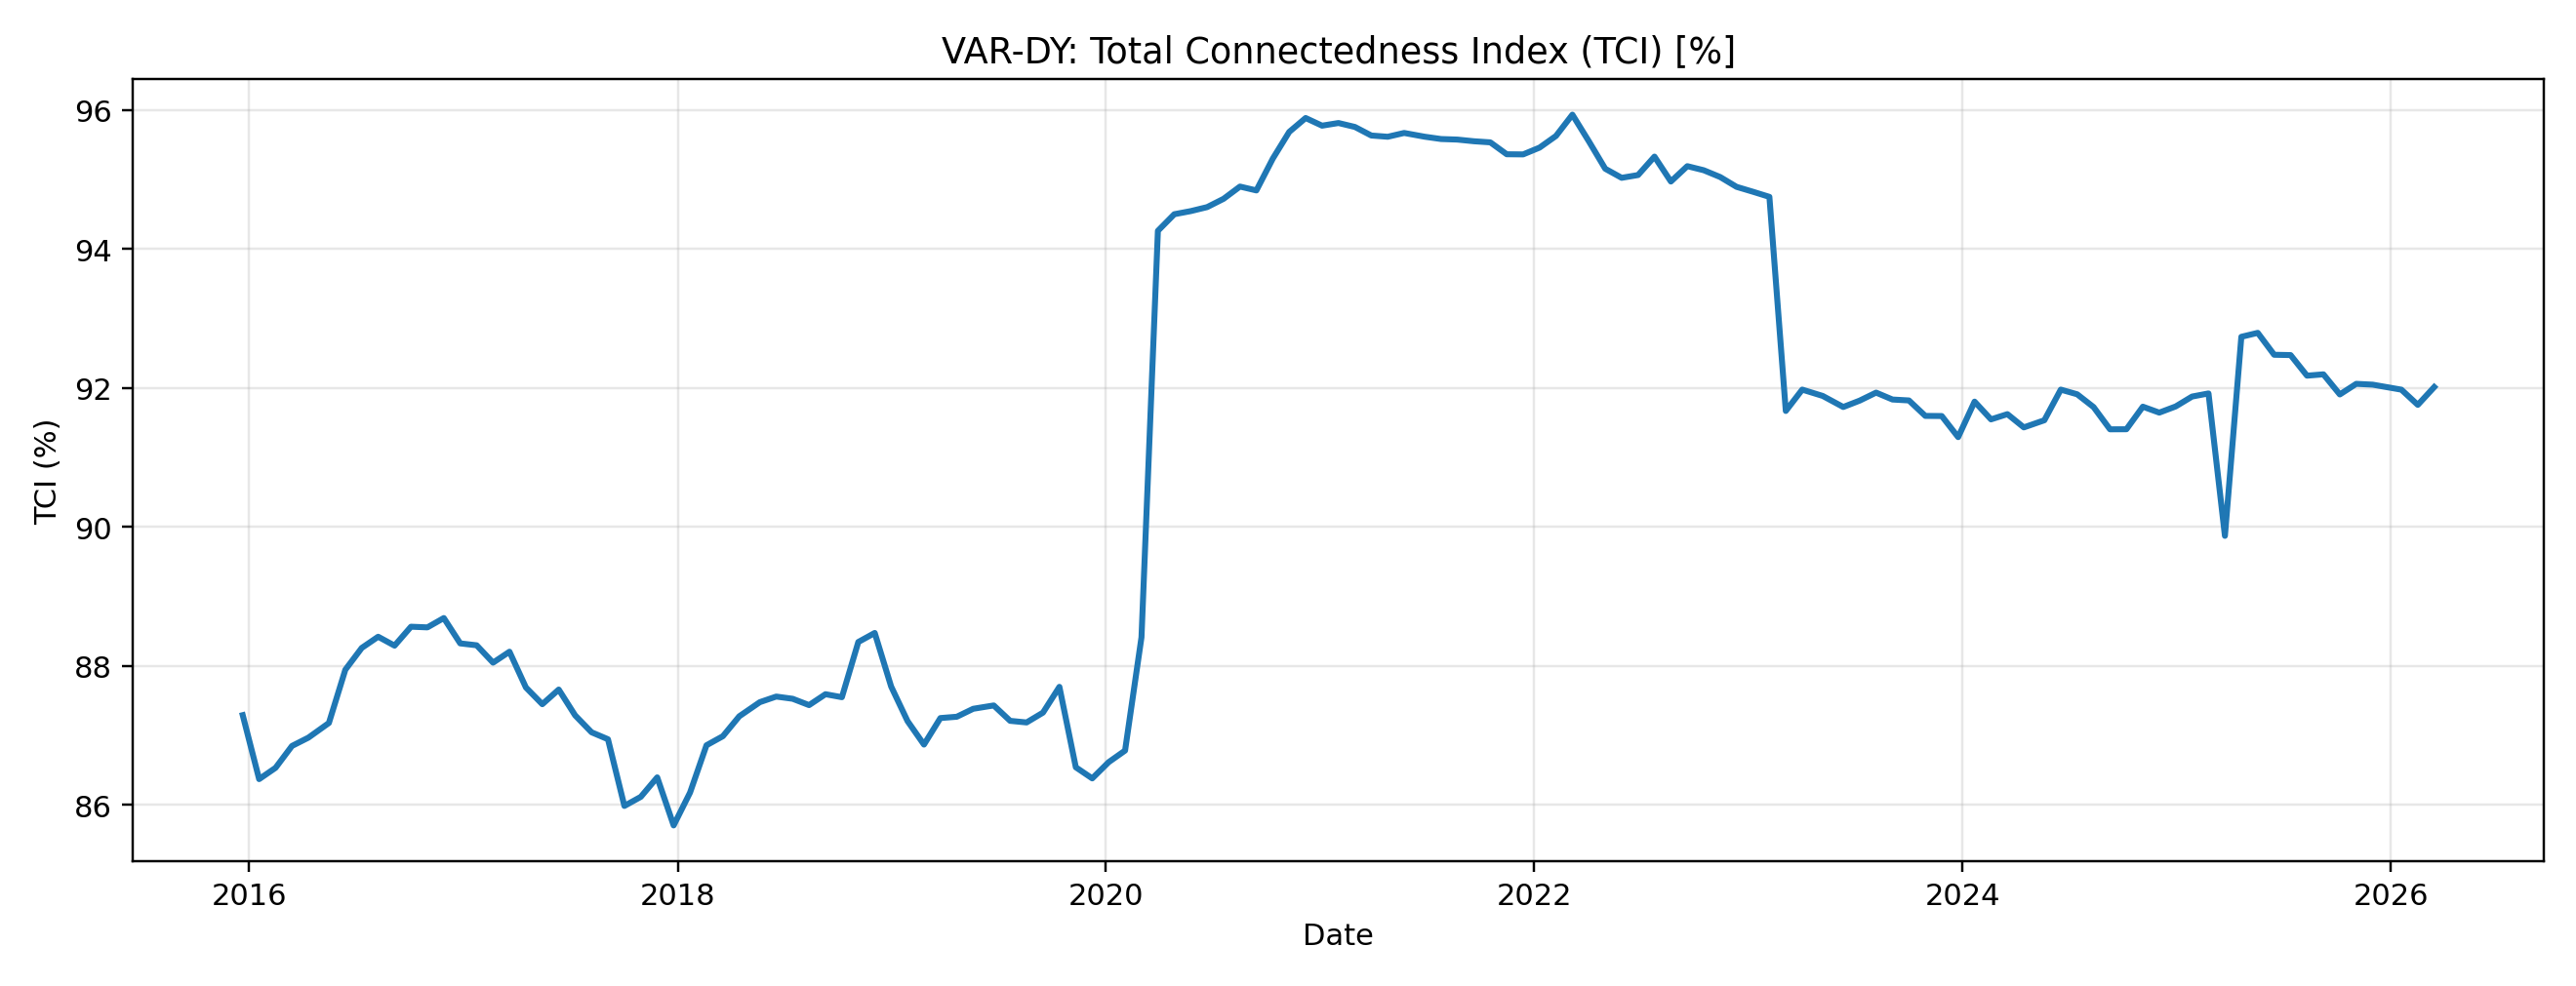
\includegraphics[width=\linewidth,height=0.66\textheight,keepaspectratio]{VAR_DY_tci_line.png}\\[-1pt]
  {\color{SlideGray}\tiny Source: rolling VAR(1)--GFEVD, $W=156$ wks, step = 4 wks, $H=10$ wks.}
 \begin{tcolorbox}[findcard=Accent,width=\linewidth]
    {\color{blue}\scriptsize\bfseries VAR-DY based TCI Dynamics 2014--2024:}\\[1pt]
    {\color{TextDark}\scriptsize We starts with VAR-DY based TCI.  Three main regimes can be detected \textbf{but TCI remains persistently high across them $\to$ may signal ``Too Interconnected/Correlated To Fail"}!}
  \end{tcolorbox}
\column{0.41\textwidth}
 \vspace{-4pt}
  \begin{tcolorbox}[findcard=Accent,width=\linewidth]
    {\color{Navy}\scriptsize\bfseries Persistently High}\\[1pt]
    {\color{TextDark}\scriptsize TCI remains in the high-80s to low-90s even in tranquil periods, showing that volatility is largely driven by common rather than idiosyncratic shocks. May imply high systemic risk.}
  \end{tcolorbox}
  \vspace{1pt}
  \begin{tcolorbox}[findcard=Red,width=\linewidth]
    {\color{Navy}\scriptsize\bfseries COVID-19 Shock}\\[1pt]
    {\color{TextDark}\scriptsize Sharp and persistent jump to about $95\%$ in early 2020: the global shock compresses idiosyncratic components and amplifies cross-institution co-movement.}
  \end{tcolorbox}
  \vspace{1pt}
  \begin{tcolorbox}[findcard=Green,width=\linewidth]
    {\color{Navy}\scriptsize\bfseries Structural Ratchet}\\[1pt]
    {\color{TextDark}\scriptsize Post-COVID TCI stabilizes above pre-2019 norms, suggesting a lasting post-COVID change in volatility linkages.  Recent  banking failures and fears in US and EU (2023-2025) do not  have a strong impact.} % https://www.linkedin.com/pulse/understanding-potential-banking-crisis-2025-john-dey-hnyfe/
  \end{tcolorbox}
\end{columns}
\end{frame}

% ── SLIDE 7b: FREQUENCY DECOMPOSITION ───────────────────────
\begin{frame}{\stag[Green]{Results} Further Decomposition of VAR-DY based TCI: Short vs.\ Long Run}
\vspace{-1pt}
\begin{columns}[T,onlytextwidth]
\column{0.57\textwidth}
  \centering
  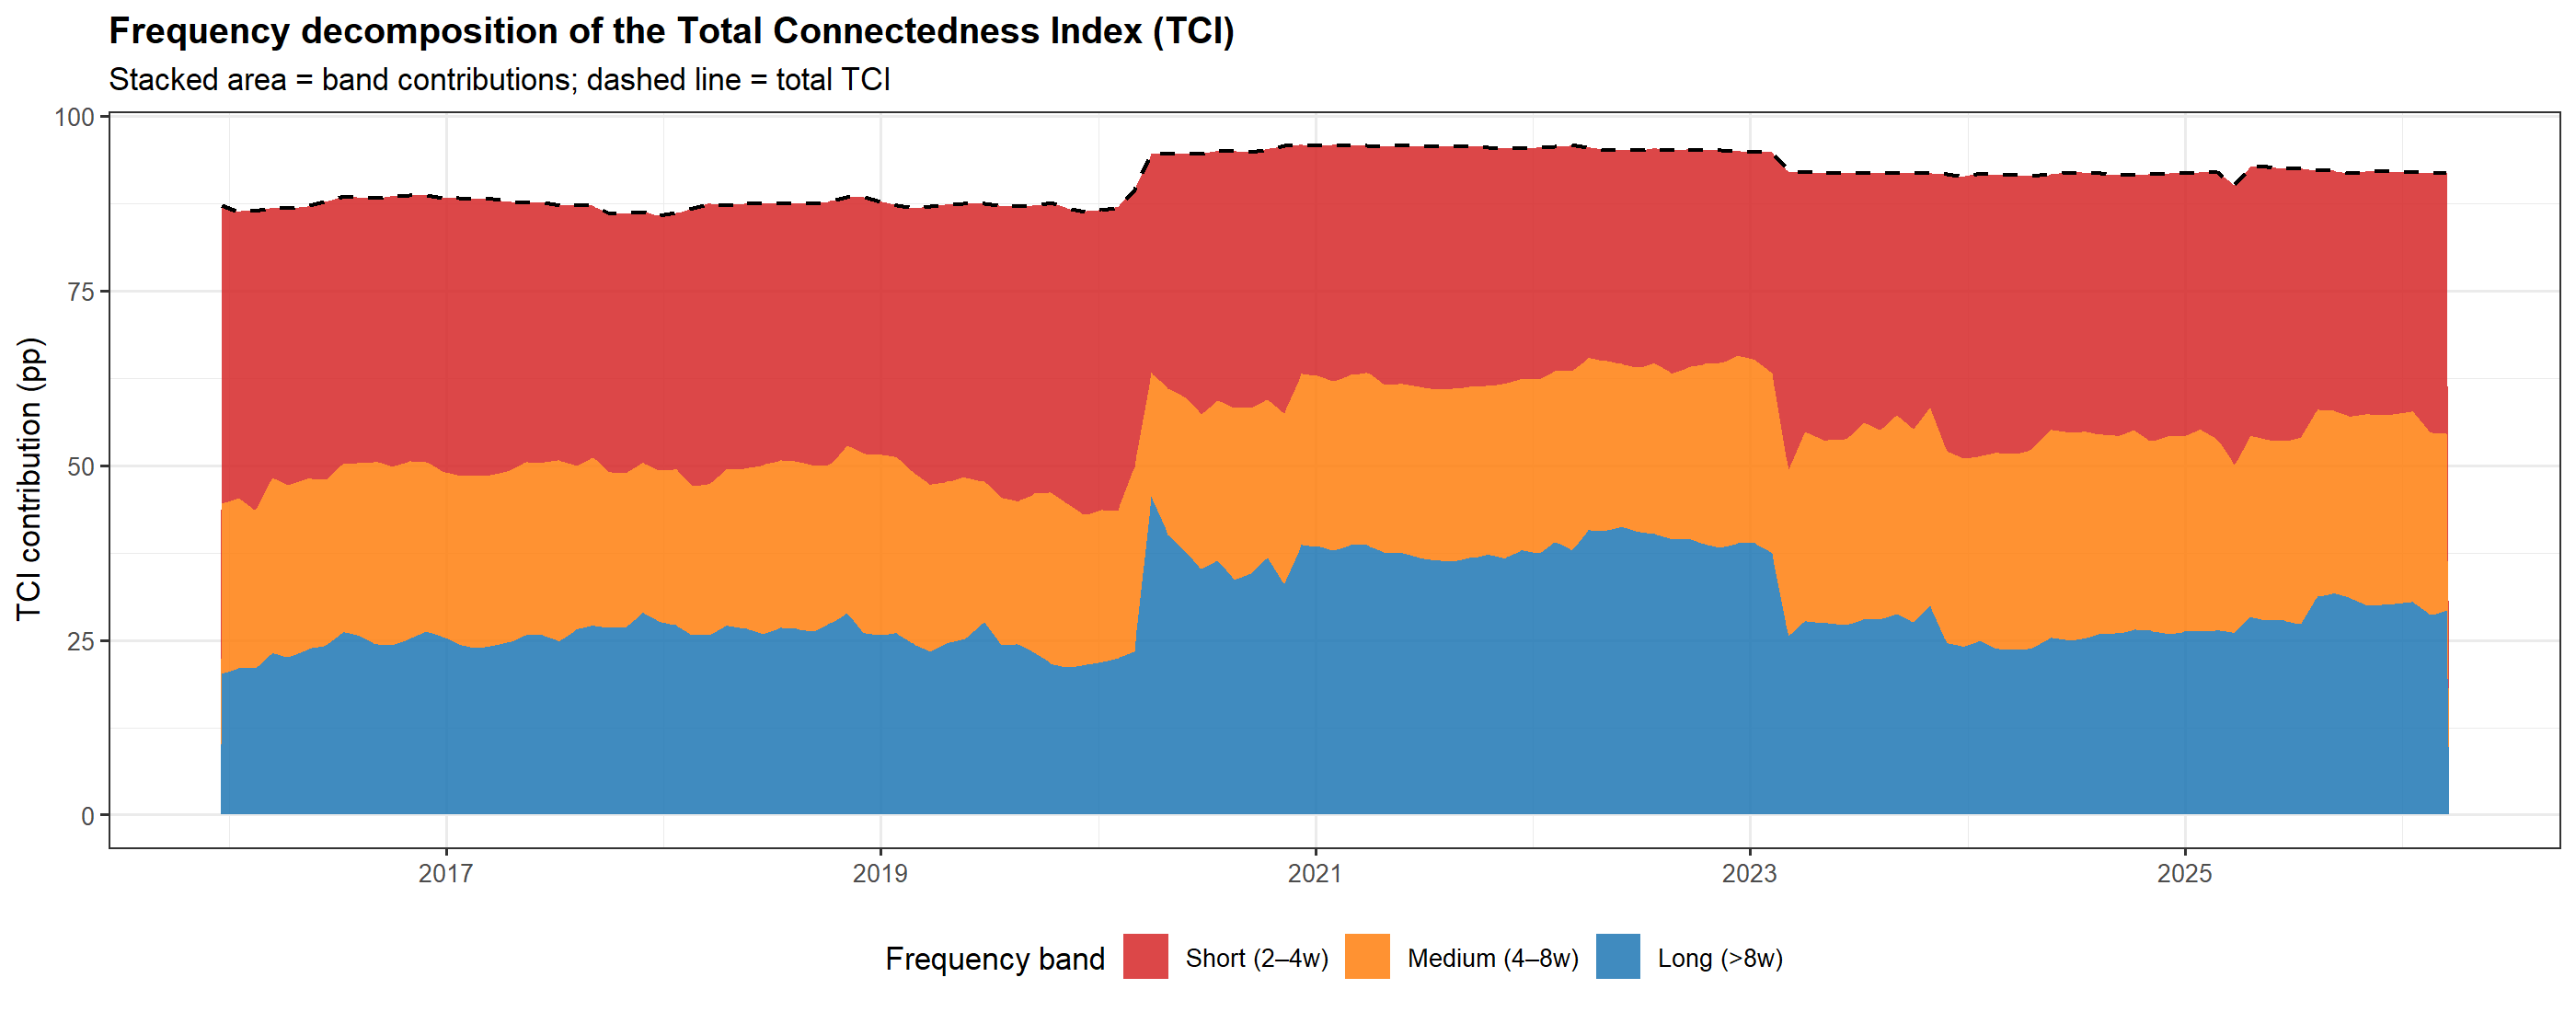
\includegraphics[width=\linewidth,height=0.66\textheight,keepaspectratio]{freq_tci_decomp.png}\\[-1pt]
  {\color{SlideGray}\tiny Stacked area = band contributions; dashed line = total TCI. Bands: Short (2--4w), Medium (4--8w), Long ($>$8w).}
  \vspace{3pt}
  \begin{tcolorbox}[findcard=blue,width=\linewidth]
    {\color{Navy}\scriptsize\bfseries Further Decomposition of TCI}\\[1pt]
    {\color{TextDark}\scriptsize 
    \textcolor{red}{TCI is decomposed into three components.......EXPLAIN THIS BRIEFLY}
    Further decomposition of the TCI reveals a more detailed asymmetric structure of volatility spillovers across frequencies.}
  \end{tcolorbox}
\vspace{-6pt}
\column{0.41\textwidth}
  \begin{tcolorbox}[findcard=Red,width=\linewidth]
    {\color{Navy}\scriptsize\bfseries Short Run Dominates in Calm Periods}\\[1pt]
    {\color{TextDark}\scriptsize 2--4 week cycles account for the largest TCI share during tranquil periods: A major portion of volatility spillovers is driven primarily by short-term fluctuations.}% $\to$ rapid interventions aimed at calming market panic may play an important role???.}%high-frequency market synchronisation.}
  \end{tcolorbox}
  \vspace{3pt}
  \begin{tcolorbox}[findcard=Accent,width=\linewidth]
    {\color{Navy}\scriptsize\bfseries COVID Expands the Long-Run Share}\\[1pt]
    {\color{TextDark}\scriptsize Long-run band ($>$8 weeks) rises from $\approx 25\%$ to $\approx 45\%$ of TCI during and after COVID: \textbf{structural rewiring in network, not just transient panic}.}
  \end{tcolorbox}
  \vspace{3pt}
  \begin{tcolorbox}[findcard=Gold,width=\linewidth]
    {\color{Navy}\scriptsize\bfseries Frequency-Heterogeneous Hubs}\\[1pt]
    {\color{TextDark}\scriptsize UBS Group (Switzerland) is the top long-run transmitter yet absent from the short-run top-5: aggregate TCI may mask/hide institutional frequency-specific roles.}
  \end{tcolorbox}
\end{columns}
\end{frame}

% ── SLIDE 8: FROM & TO ────────────────────────────────────────
\begin{frame}{\stag[Green]{Results} Directional Connectedness Rank: Major Receivers \& Emitters}
\vspace{-1pt}
\begin{columns}[T,onlytextwidth]
\column{0.49\textwidth}
  \centering
  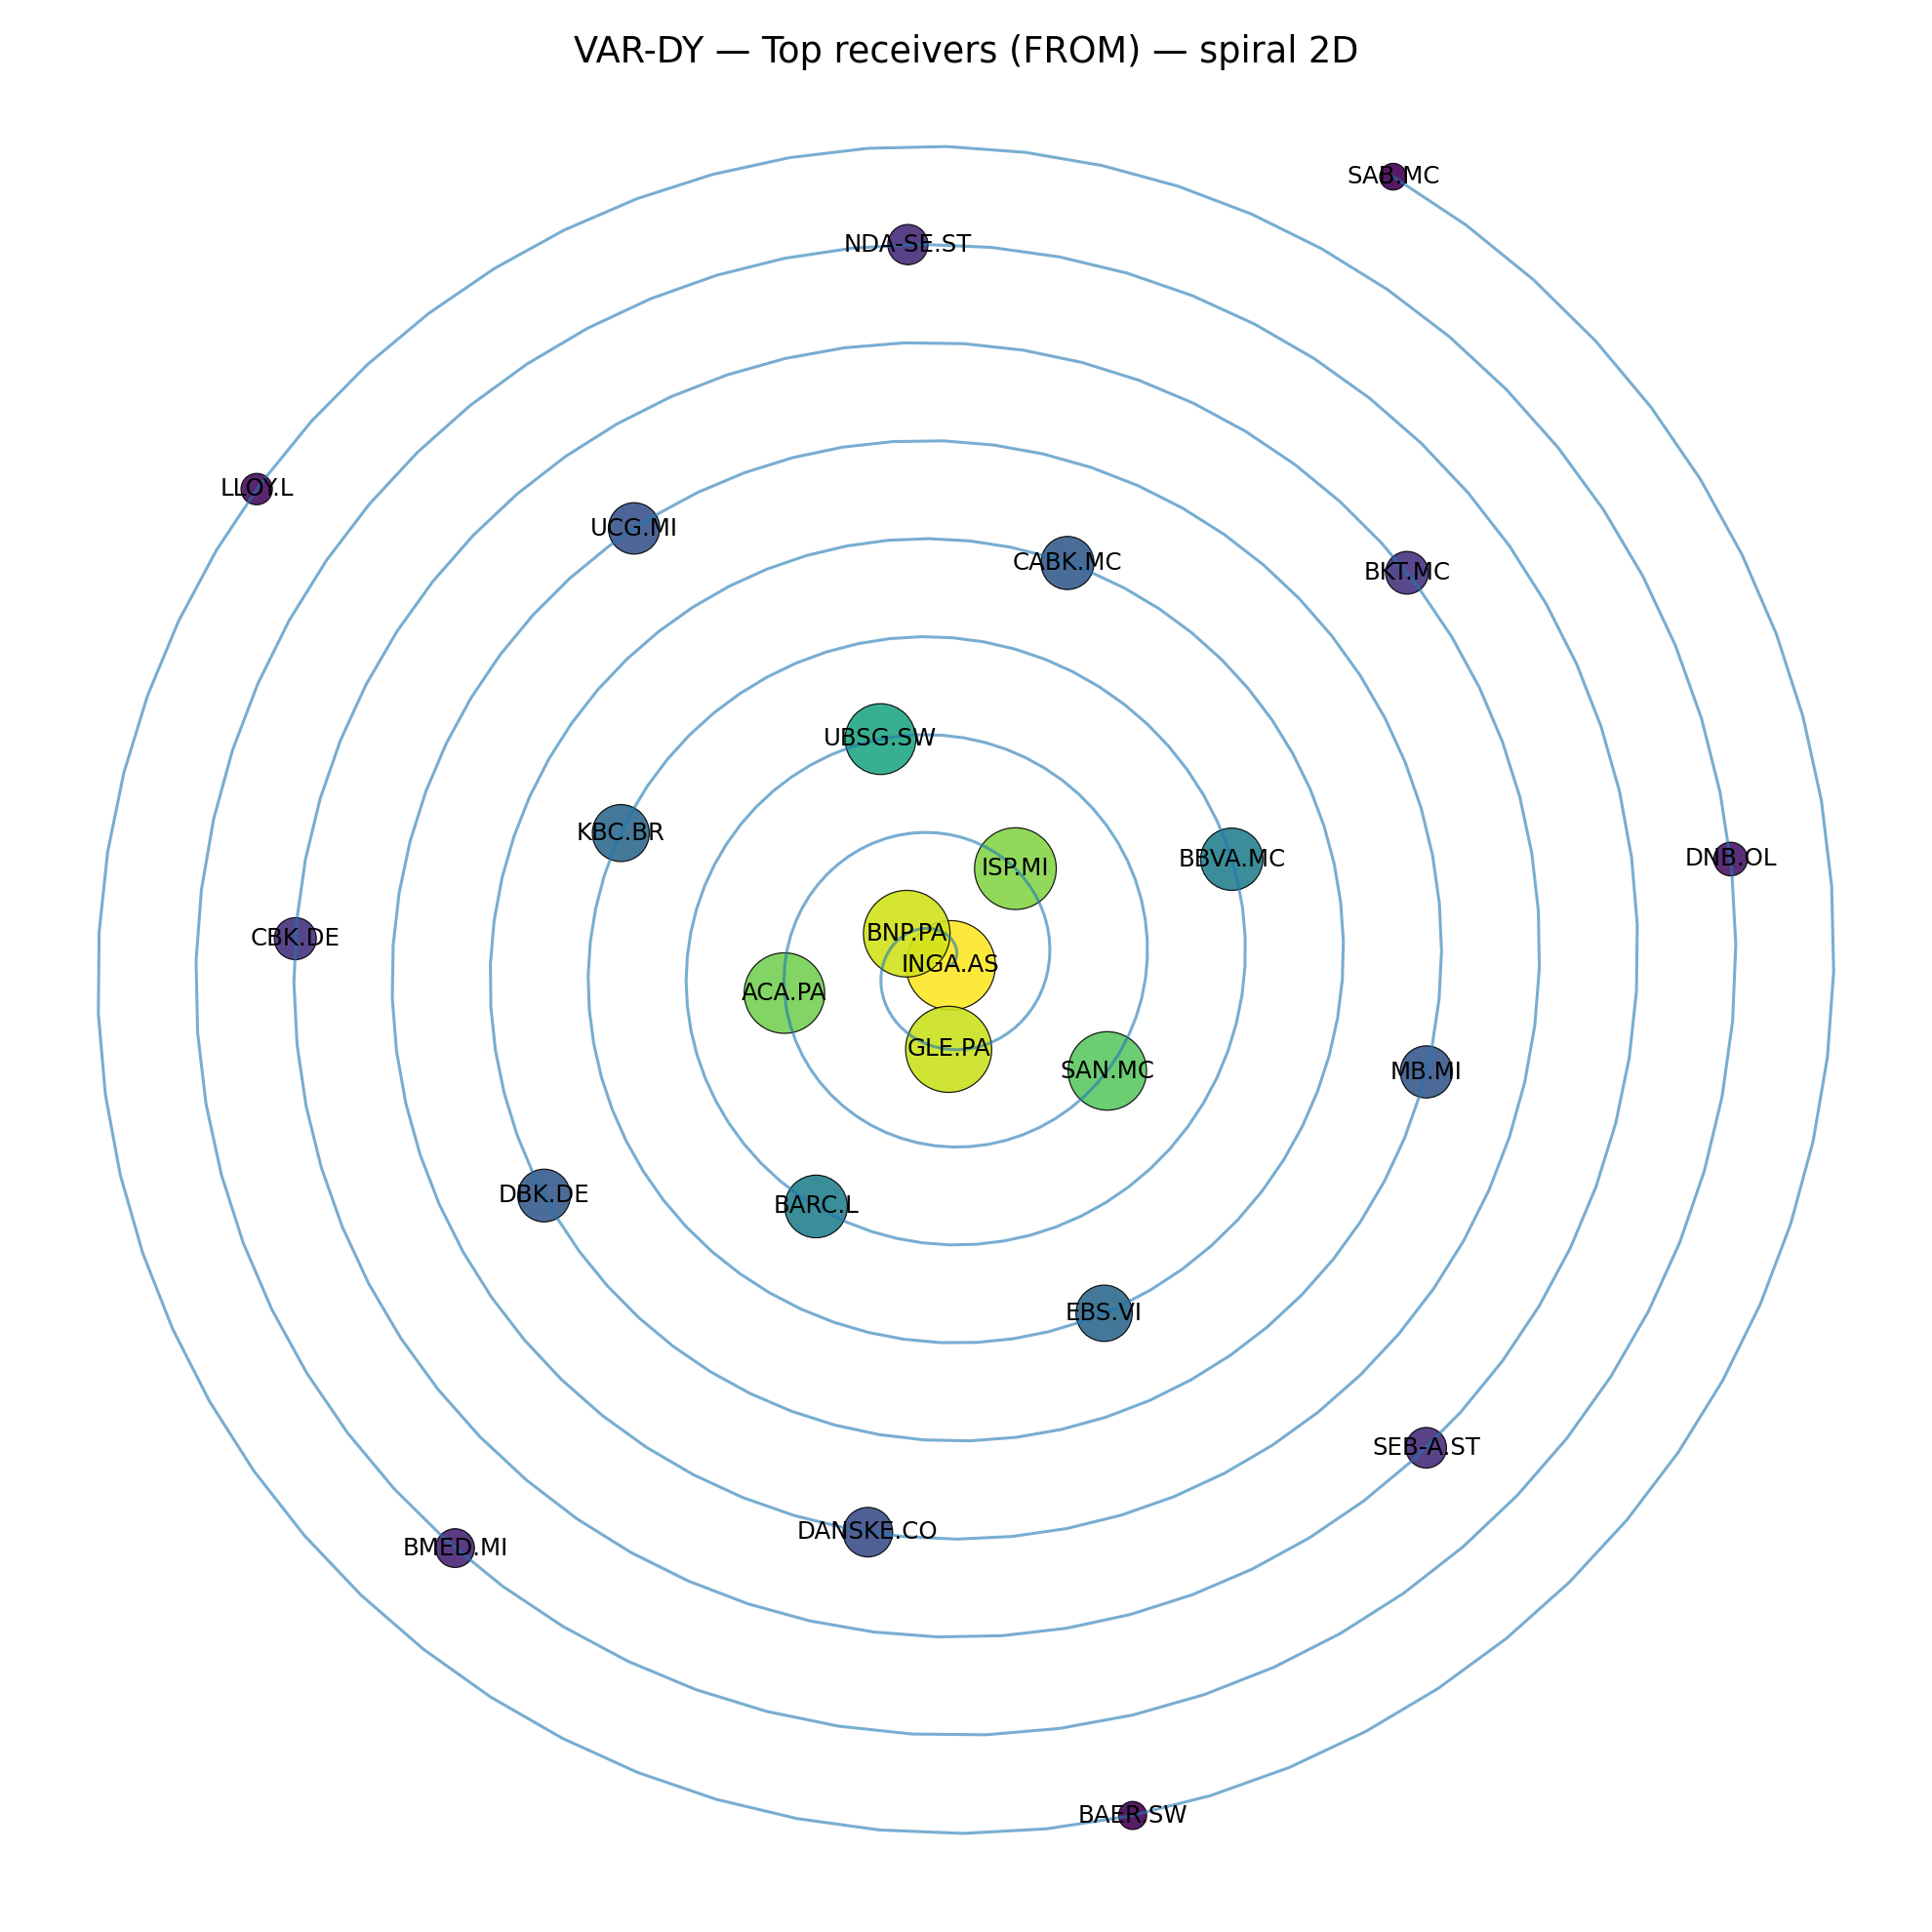
\includegraphics[width=\linewidth,height=0.65\textheight,keepaspectratio]{VAR_DY_helix_FROM_spiral.png}

\column{0.49\textwidth}
  \centering
  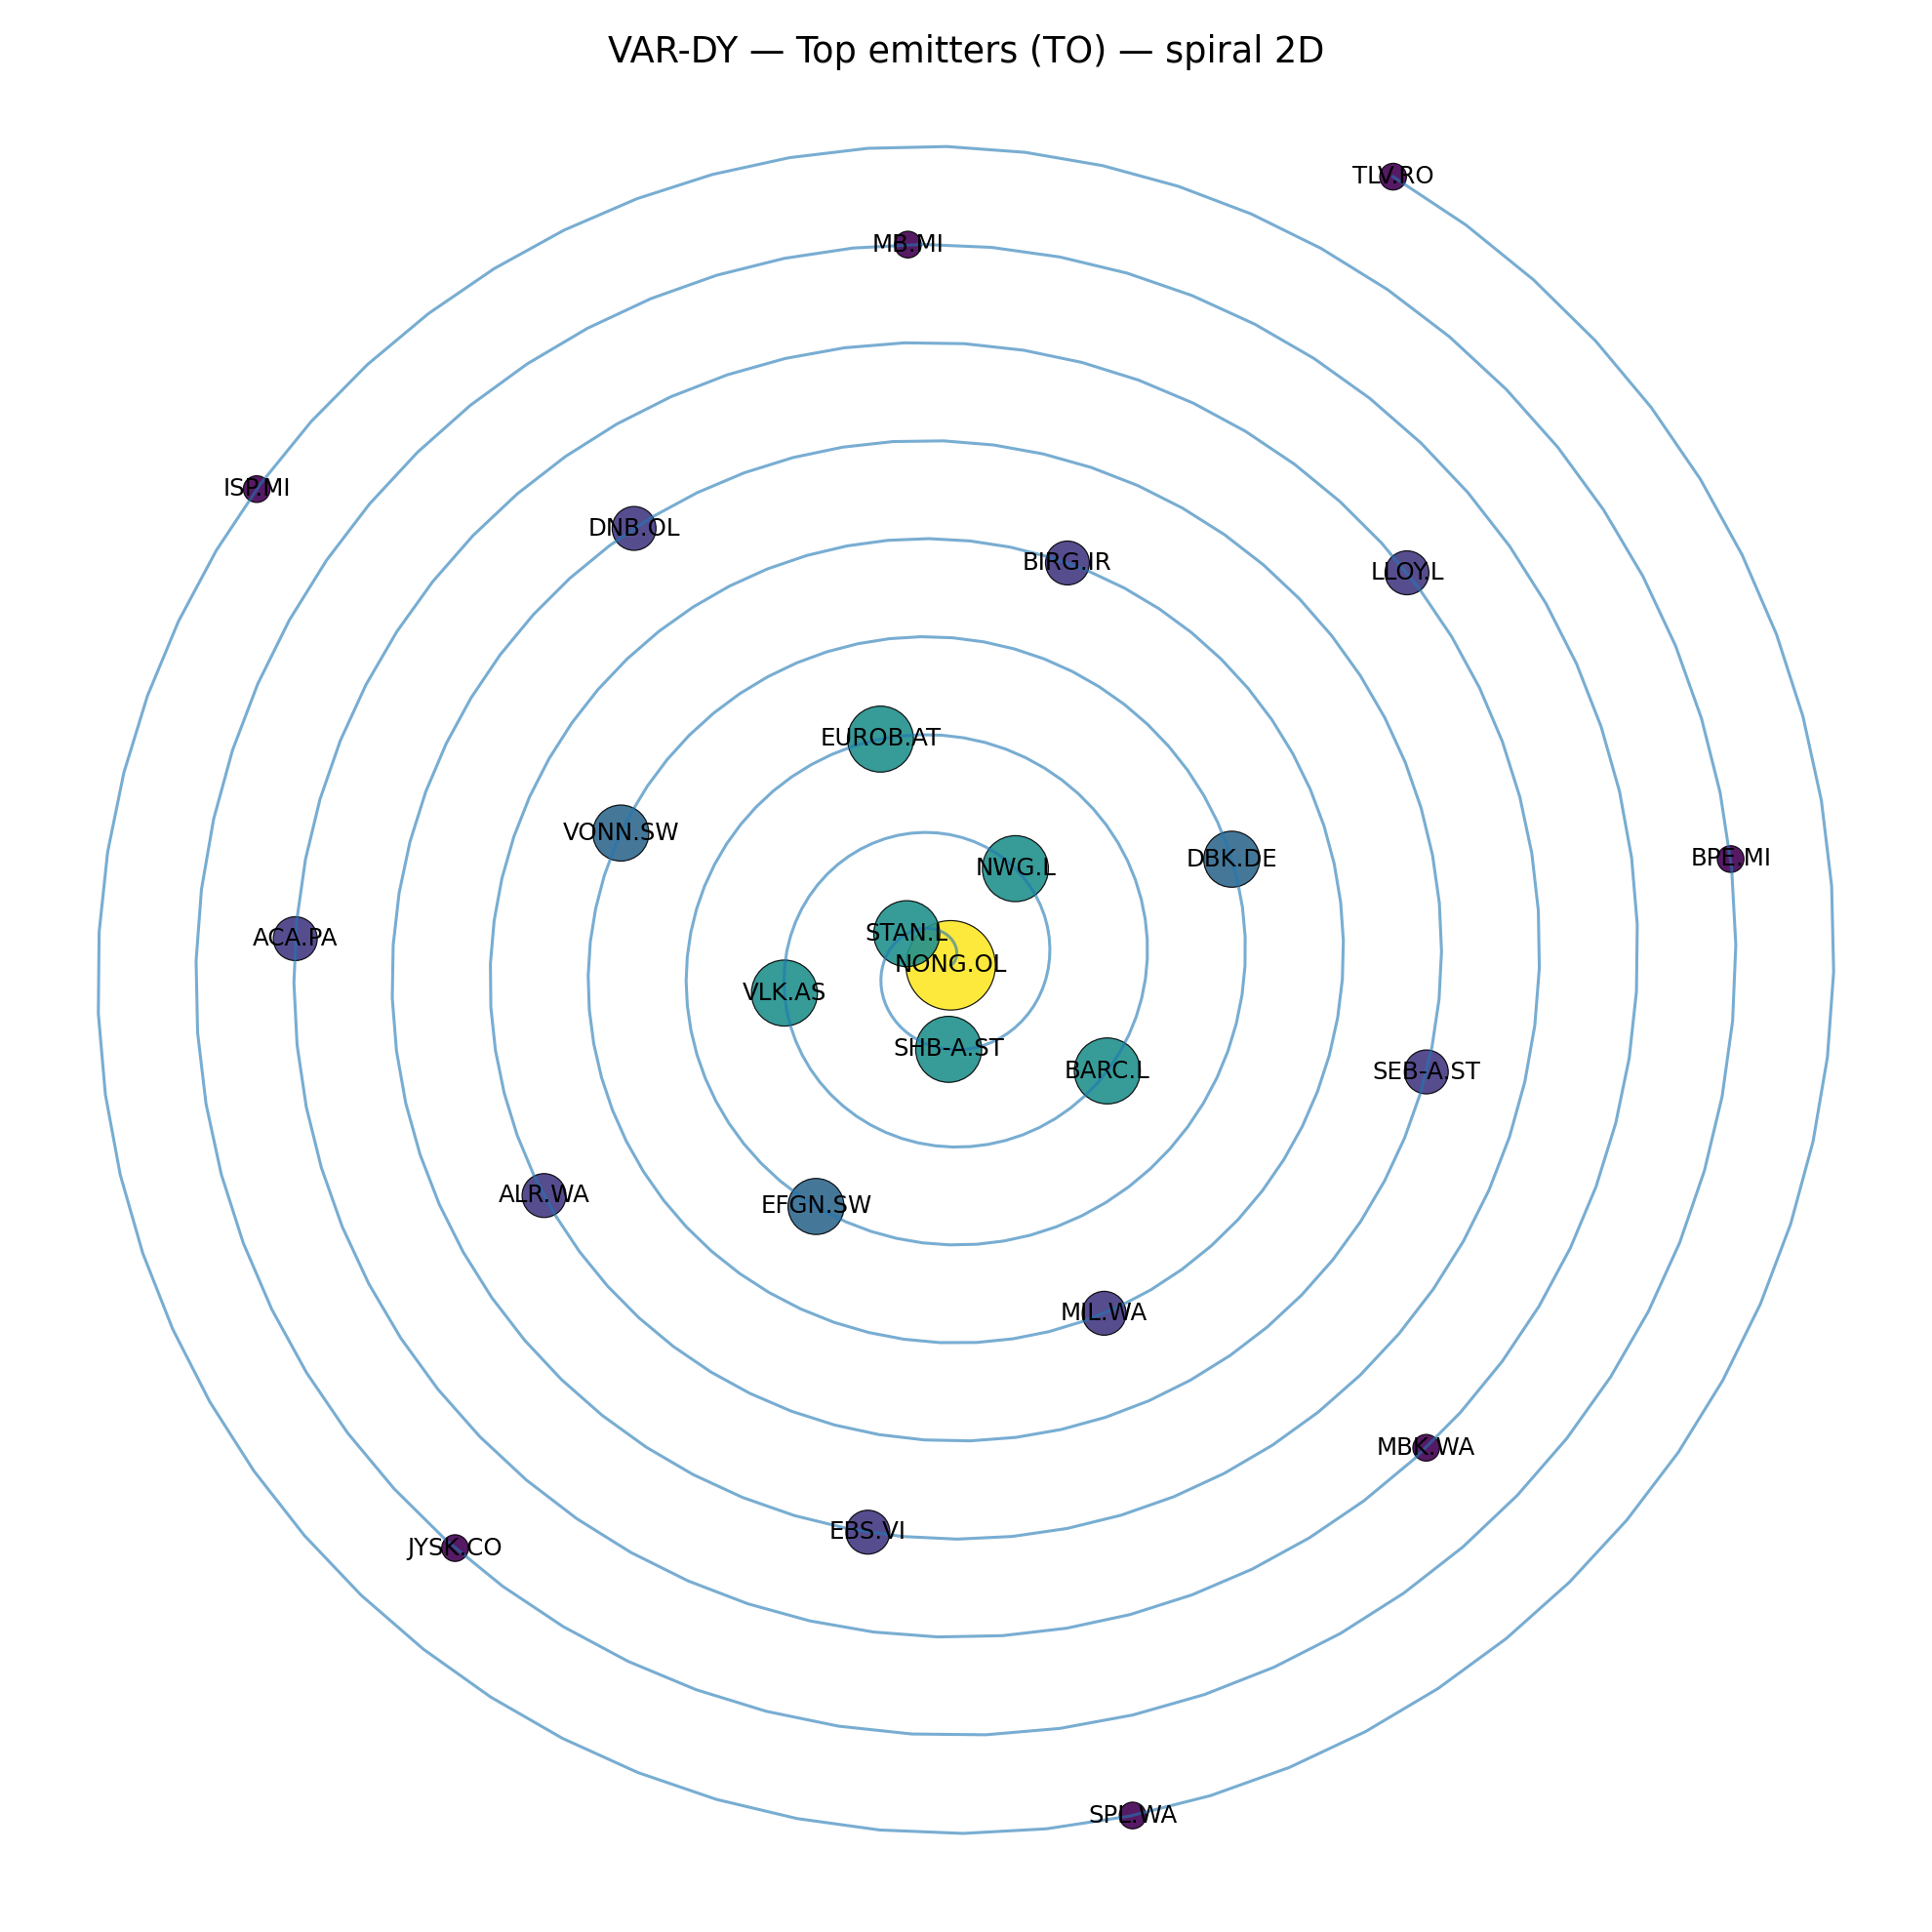
\includegraphics[width=\linewidth,height=0.65\textheight,keepaspectratio]{VAR_DY_helix_TO_spiral.png}
\end{columns}

\vspace{2pt}
\begin{tcolorbox}[navybox]
  \scriptsize\centering   \textbf{\color{Gold}While TCI is high and the network is not sparse, the roles played by individual banks differ.}\\
  \textbf{\color{Gold}Receivers core:}  \scriptsize BNP Paribas (FR) · Société Générale (FR)· ING Group (NL) · Santander (ES) · UBS (SW)\\ \hspace{0.8em}
  \textbf{\color{Gold}Emitters core:}  \scriptsize 
  Société Générale (FR) . Bankinter (ES); Raiffeisen (AT); Skandinaviska Enskilda Banken (SE); KBC Group (BE)
%Bank codes: GLE.PA · BKT.MC · TPEIR.AT · SEB-A.ST · KBC.BR
\end{tcolorbox}
\end{frame}

% ── SLIDE 9: NET SPILLOVERS ───────────────────────────────────
\begin{frame}{\stag[Green]{Results} In-Depth Analysis: Net Transmitters vs.\ Net Receivers}
\vspace{-8pt}
\begin{columns}[T,onlytextwidth]
\column{0.43\textwidth}
  \begin{tcolorbox}[whitebox=Accent]
    {\color{Navy}\small\bfseries Definition}\\[1pt]
    {\color{TextDark}\scriptsize Recalling net spillover:}
    \[
    C_i^{\mathrm{net}}(H)=
    C_{i\rightarrow\bullet}(H)-C_{i\leftarrow\bullet}(H)
    \]
    \[
    C_i^{\mathrm{net}}>0 \Rightarrow \text{net transmitter}
    \]
    \[
    C_i^{\mathrm{net}}<0 \Rightarrow \text{net receiver}
    \]
    {\color{TextDark}\scriptsize Time-averaged net spillover:}
    \[
    \bar C_i^{\mathrm{net}}
    =
    \bar C_{i\rightarrow\bullet}-\bar C_{i\leftarrow\bullet}
    \]
  \end{tcolorbox}
  %\vspace{2pt}
  \begin{tcolorbox}[whitebox=Gold]
    {\color{Navy}\small\bfseries Macroprudential implication}\\[1pt]
    {\color{TextDark}\scriptsize Peripheral net transmitters are  outward stress channels and deserve closer cross-border supervisory attention. Banks having a dual role may complicate efforts to mitigate spillover effects $\to$ \textbf{Not simply ``Too Big To Fail"} or \textbf{``Too Small To Matter"!}}
  \end{tcolorbox}

\column{0.54\textwidth}
  \begin{tcolorbox}[findcard=Red,width=\linewidth]
    {\color{Navy}\scriptsize\bfseries Peripheral \& Smaller Market Banks}\\[1pt]
    {\color{TextDark}\scriptsize From peripheral or smaller markets but typically found as \textbf{net transmitters}: volatility propagates outward to the rest of the system.}
  \end{tcolorbox}
  \vspace{3pt}
  \begin{tcolorbox}[findcard=Accent,width=\linewidth]
    {\color{Navy}\scriptsize\bfseries Large Western European Banks}\\[1pt]
    {\color{TextDark}\scriptsize Structural \textbf{net receivers}: they receive more volatility from the system than they transmit.}
  \end{tcolorbox}
  \vspace{3pt}
  \begin{tcolorbox}[findcard=Gold,width=\linewidth]
    {\color{Navy}\scriptsize\bfseries Dual-role Institutions}\\[1pt]
    {\color{TextDark}\scriptsize Several large cross-border banks appear among both \textbf{top/key} receivers and top emitters, reflecting their role as both targets and amplifiers of systemic volatility.}
  \end{tcolorbox}
\end{columns}
\end{frame}

% ── SLIDE 10: DCC DEPENDENCE ──────────────────────────────────
\begin{frame}{\stag[Green]{Results} DCC--GARCH: Correlation Dynamics \& Network Centrality}
\vspace{-10pt}
\begin{columns}[T,onlytextwidth]
\column{0.42\textwidth}
  \begin{tcolorbox}[mathbox]
    {\color{Gold}\bfseries\scriptsize Mean absolute DCC correlation (DCC mean):}\\[2pt]
    $\displaystyle\bar\rho_t=\frac{2}{N(N-1)}\sum_{i<j}\lvert\rho_{ij,t}\rvert$.
    $\rho_{ij,t}$ is the correlaiton between banks $i, j$ implied by the DCC-GARCH model.
  \end{tcolorbox}
  \vspace{1pt}
  \begin{tcolorbox}[findcard=Accent,width=\linewidth]
    {\color{Navy}\scriptsize\bfseries Structurally Interdependent}\\[1pt]
    {\color{TextDark}\scriptsize $\bar\rho_t\approx0.30$--$0.35$ in calm periods: EU financial equities remain co-dependent throughout the sample.}
  \end{tcolorbox}\vspace{1pt}
  \begin{tcolorbox}[findcard=Red,width=\linewidth]
    {\color{Navy}\scriptsize\bfseries COVID-19 Spike}\\[1pt]
    {\color{TextDark}\scriptsize  $\bar\rho_t$ jumps above 0.50 in 2020 and stays elevated; timing closely matches the VAR-based TCI surge.}
  \end{tcolorbox}\vspace{1pt}
  \begin{tcolorbox}[findcard=Gold,width=\linewidth]
    {\color{Navy}\scriptsize\bfseries Stable Core of DCC Hubs}\\[1pt]
    {\color{TextDark}\scriptsize BNP Paribas (FR), Société Générale (FR), ING Group (NL), Intesa Sanpaolo (IT), KBC Group (BR), Banco Santander (ES), UBS Group AG (SW).}% remain persistently central.}
    
    %BNP.PA, GLE.PA, INGA.AS, ISP.MI, KBC.BR, SAN.MC and UBSG.SW remain persistently central.}
  \end{tcolorbox}
\vspace{2pt}
\column{0.56\textwidth}
  \centering
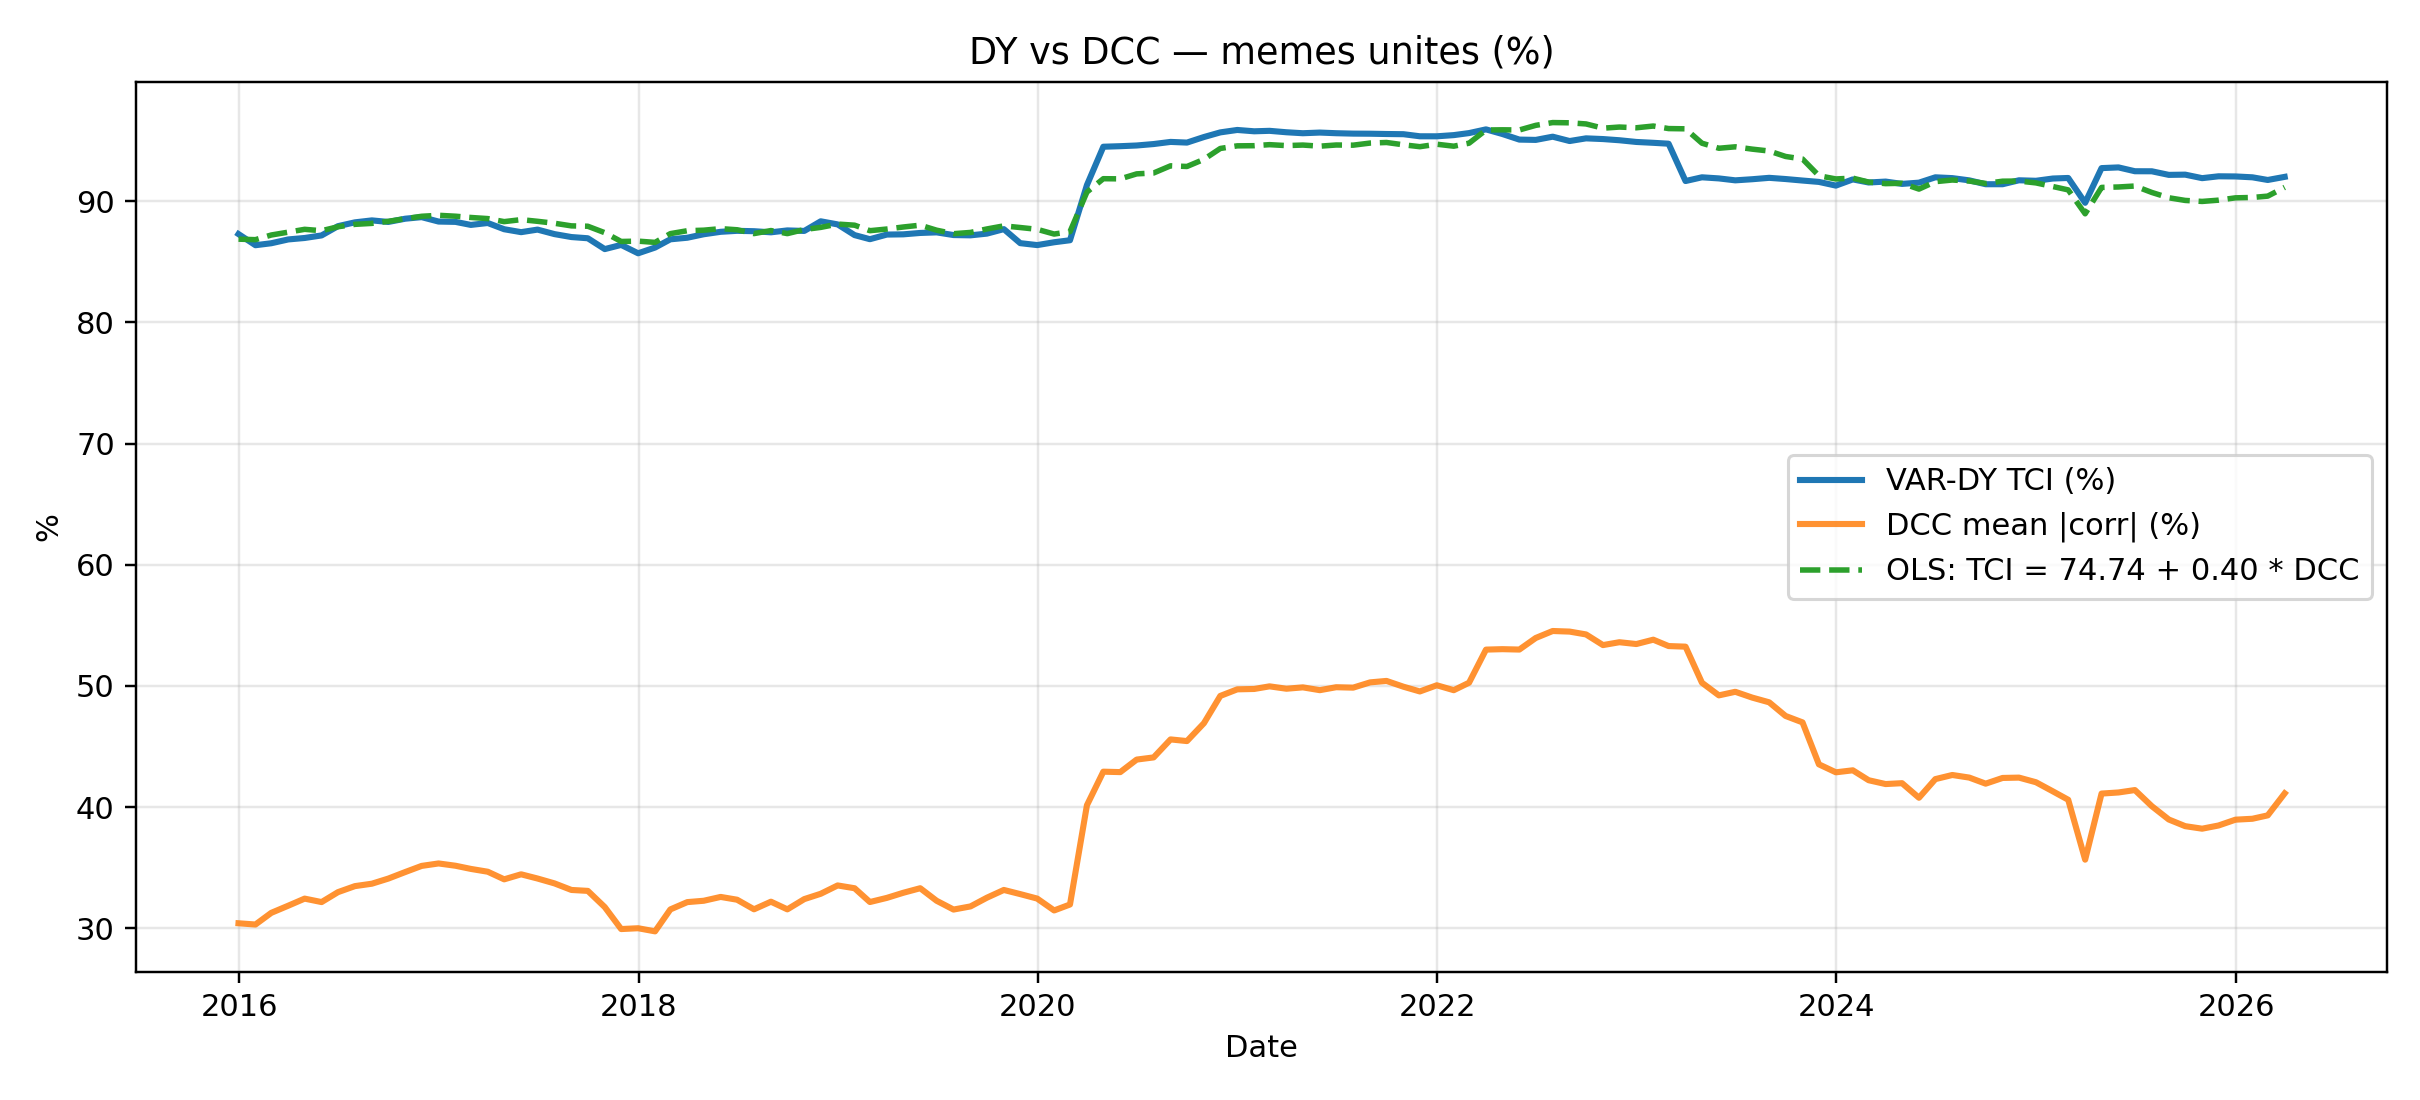
\includegraphics[width=\linewidth,height=0.68\textheight,keepaspectratio]{DY_DCC_levels_reg.png}

\begin{tcolorbox}[findcard=blue,width=\linewidth]
    {\color{Navy}\scriptsize\bfseries  DCC mean vs.  VAR-DY based TCI }\\[1pt]
    {\color{TextDark}\scriptsize Overall, the DCC-GARCH-based TCI closely replicates the VAR-DY-based TCI (see also the next slide).\\ However, while the VAR-DY-based network is directed (hence, richer information), the DCC-GARCH-based network is undirected.}% remain persistently central.}
    \end{tcolorbox}  
    \end{columns}
\end{frame}

% ── SLIDE 11: DY vs DCC ───────────────────────────────────────
\begin{frame}{\stag[Green]{Results} VAR--DY vs.\ DCC--GARCH: Convergent Systemic Risk Signals from TCI Perspective}
\vspace{-1pt}
\begin{columns}[T,onlytextwidth]
\column{0.56\textwidth}
  \centering
  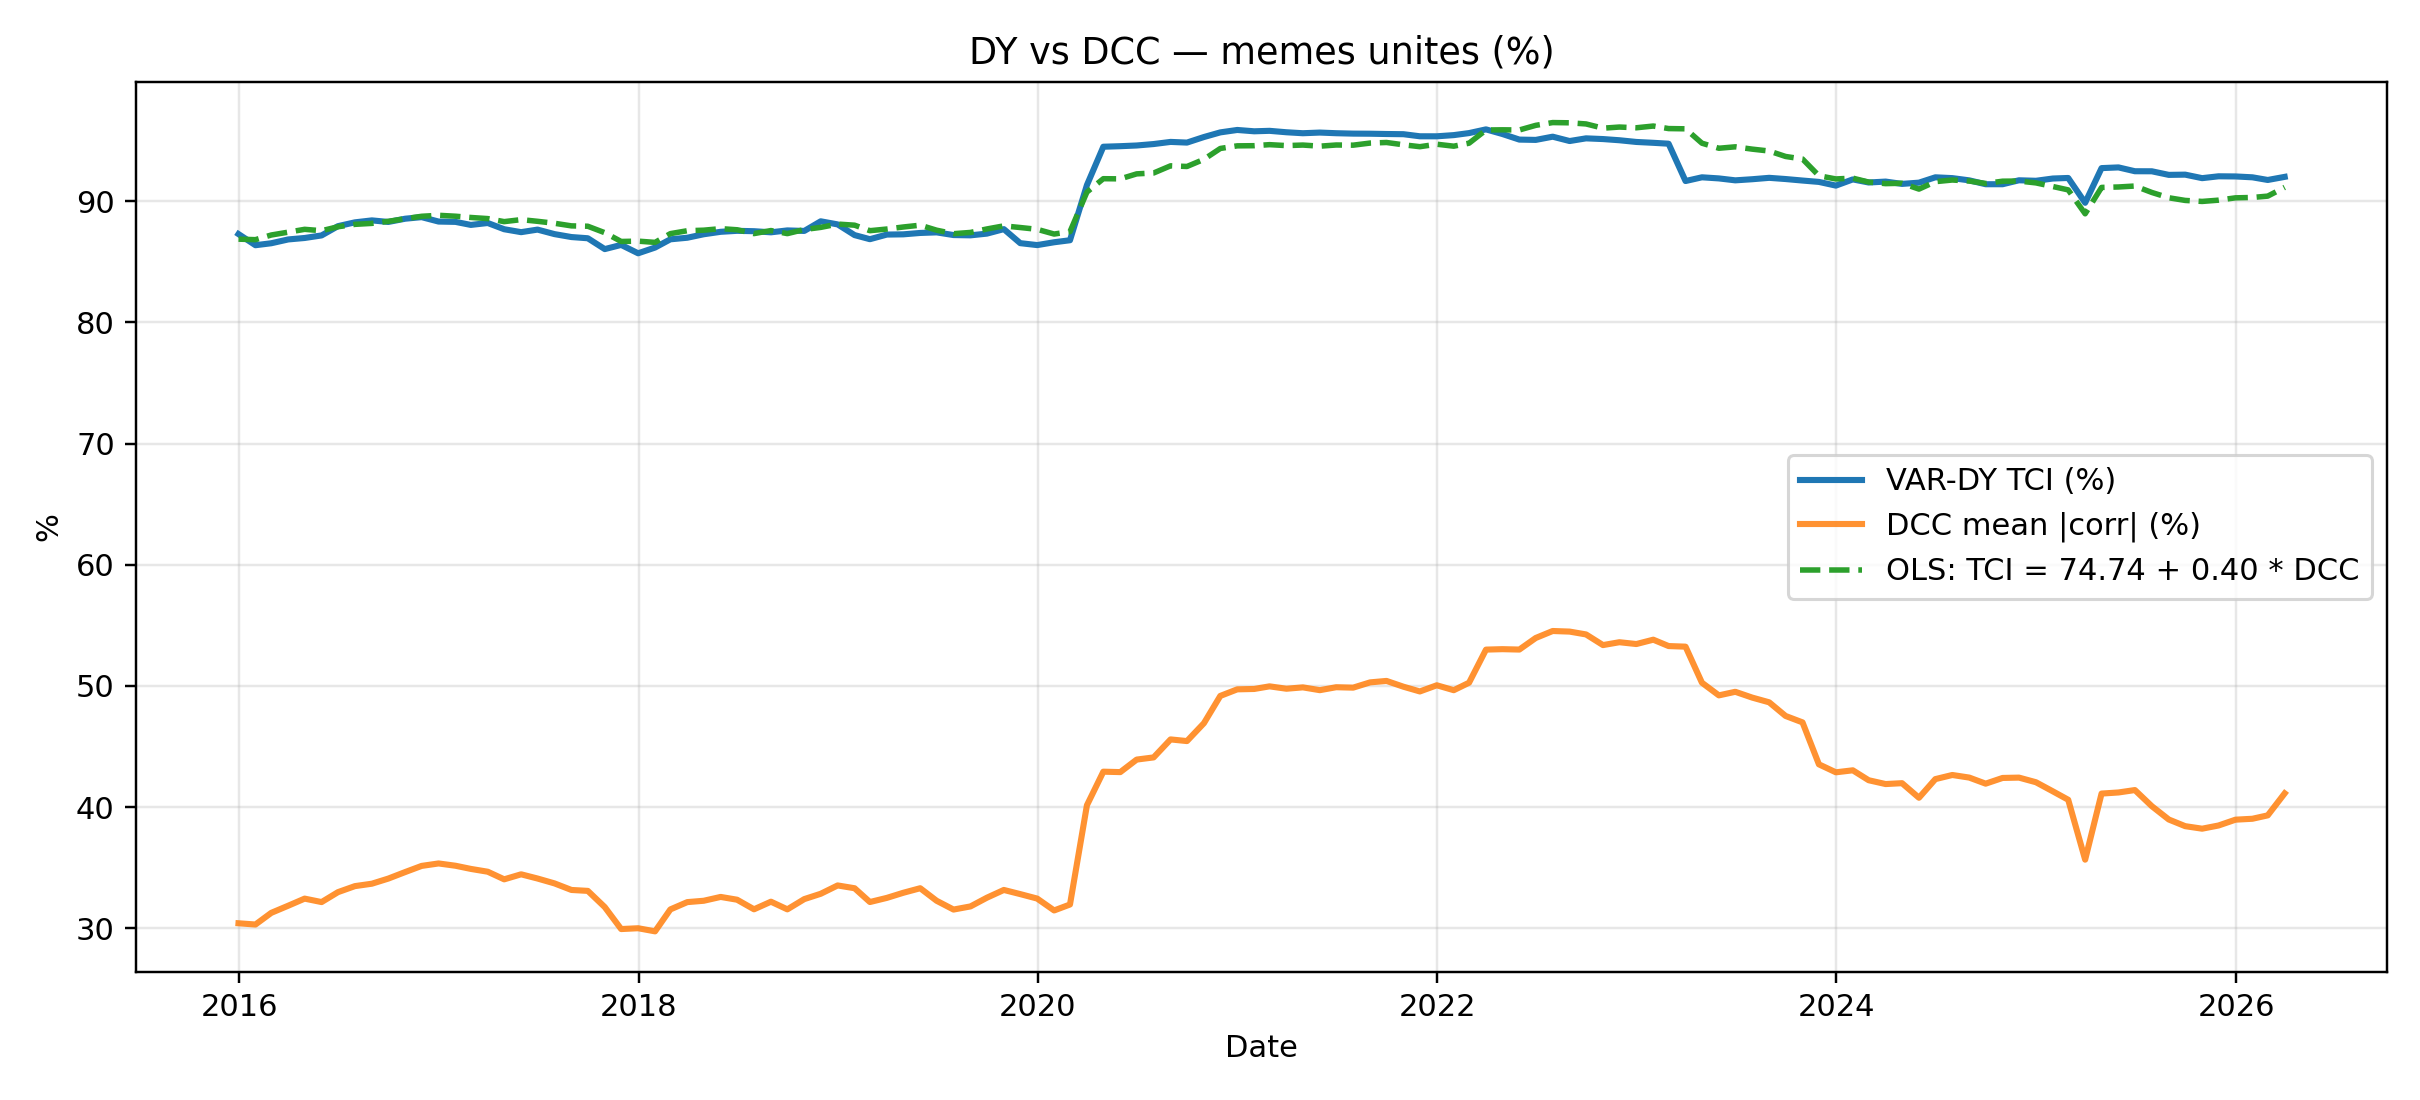
\includegraphics[width=\linewidth,height=0.44\textheight,keepaspectratio]{DY_DCC_levels_reg.png}

\column{0.42\textwidth}
  \centering
  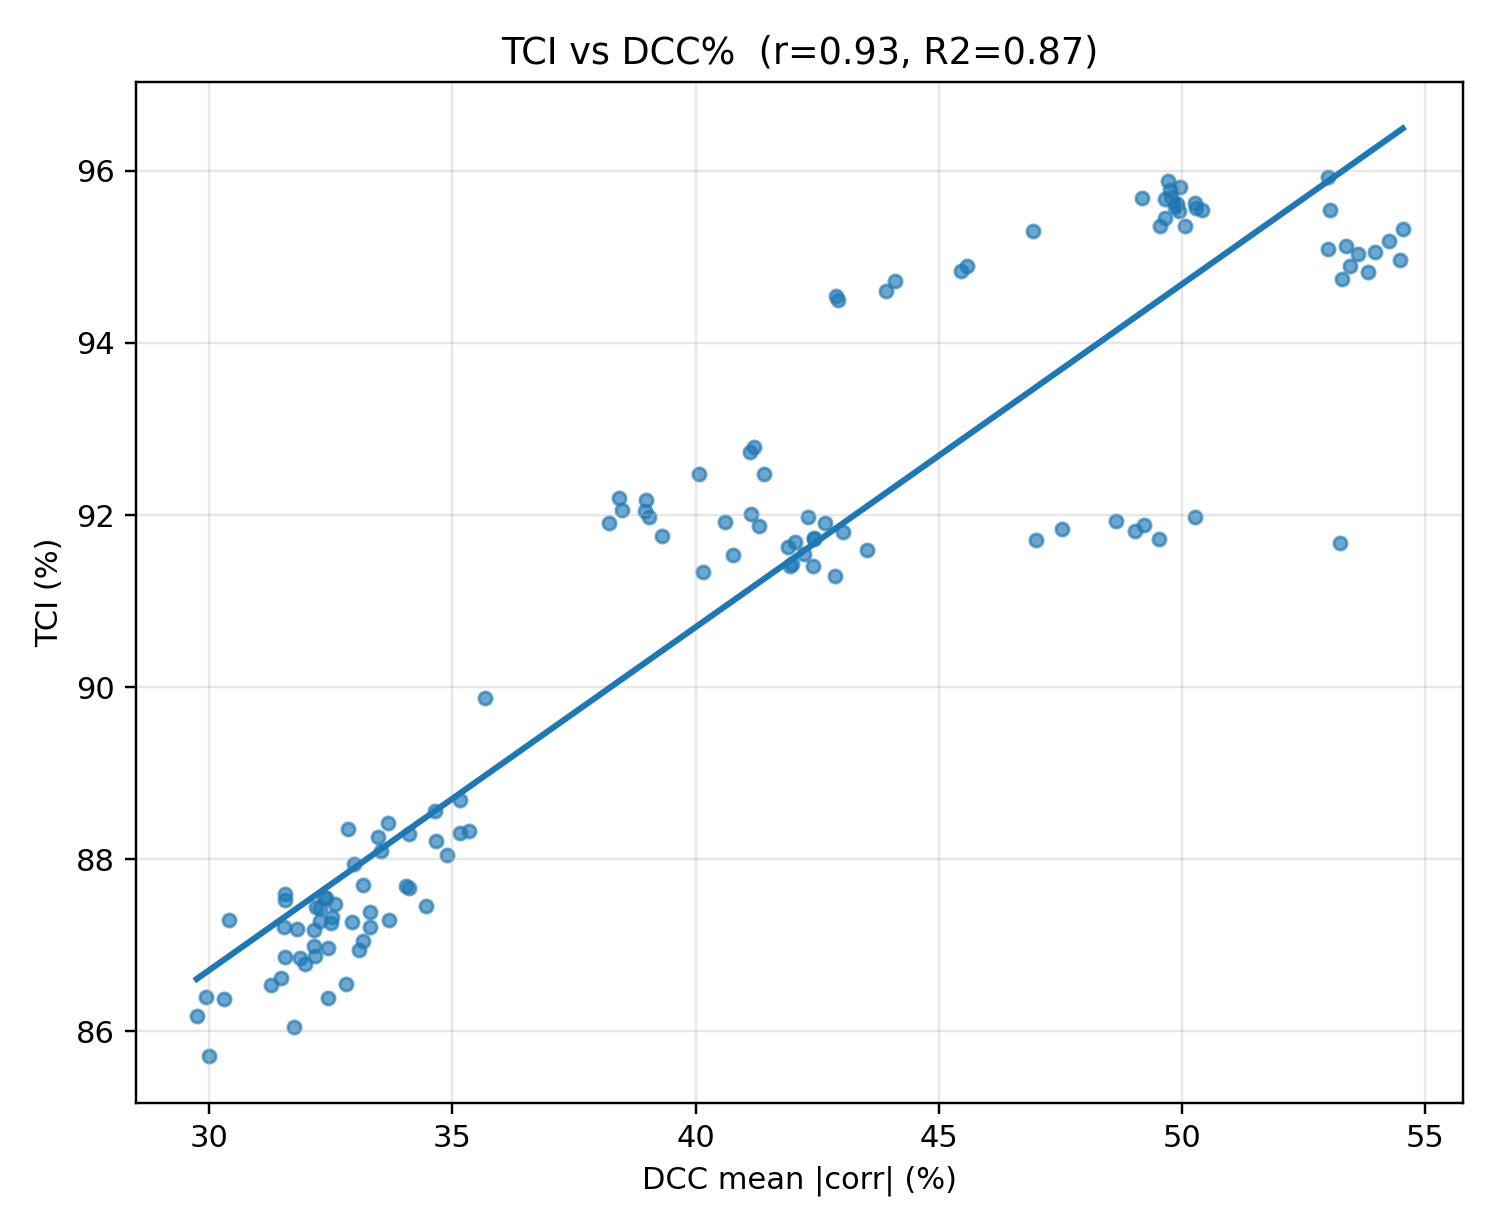
\includegraphics[width=\linewidth,height=0.44\textheight,keepaspectratio]{DY_DCC_scatter_reg.png}
\end{columns}

\vspace{3pt}
\begin{columns}[T,onlytextwidth]
\column{0.32\textwidth}
\begin{tcolorbox}[whitebox=Accent]
  {\color{Accent}\large\bfseries $R^2\approx0.88$}\\[1pt]
  {\color{TextDark}\scriptsize Near-linear association across market regimes despite different model assumptions.}
\end{tcolorbox}

\column{0.32\textwidth}
\begin{tcolorbox}[whitebox=Green]
  {\color{Green}\large\bfseries $r\approx0.94$}\\[1pt]
  {\color{TextDark}\scriptsize Pearson correlation between rolling $\mathrm{TCI}_w$ and mean absolute DCC.}
\end{tcolorbox}

\column{0.32\textwidth}
\begin{tcolorbox}[whitebox=Gold]
  {\color{Gold}\normalsize\bfseries DCC leads TCI by $\sim\!1$ window}\\[1pt]
  {\color{TextDark}\scriptsize Cross-correlation peaks at lag $-1$: DCC provides early-warning information.}
\end{tcolorbox}
\end{columns}
\end{frame}

% ── SLIDE 11b: CONNECTEDNESS REGIMES   DELETED THIS SLIDE

%\begin{frame}{\stag[Green]{Results} Connectedness Regimes: $k$-Means \textcolor{red} {????} on GFEVD Feature Vectors}
%\vspace{-1pt}
%\begin{columns}[T,onlytextwidth]
%\column{0.57\textwidth}
%  \centering
  %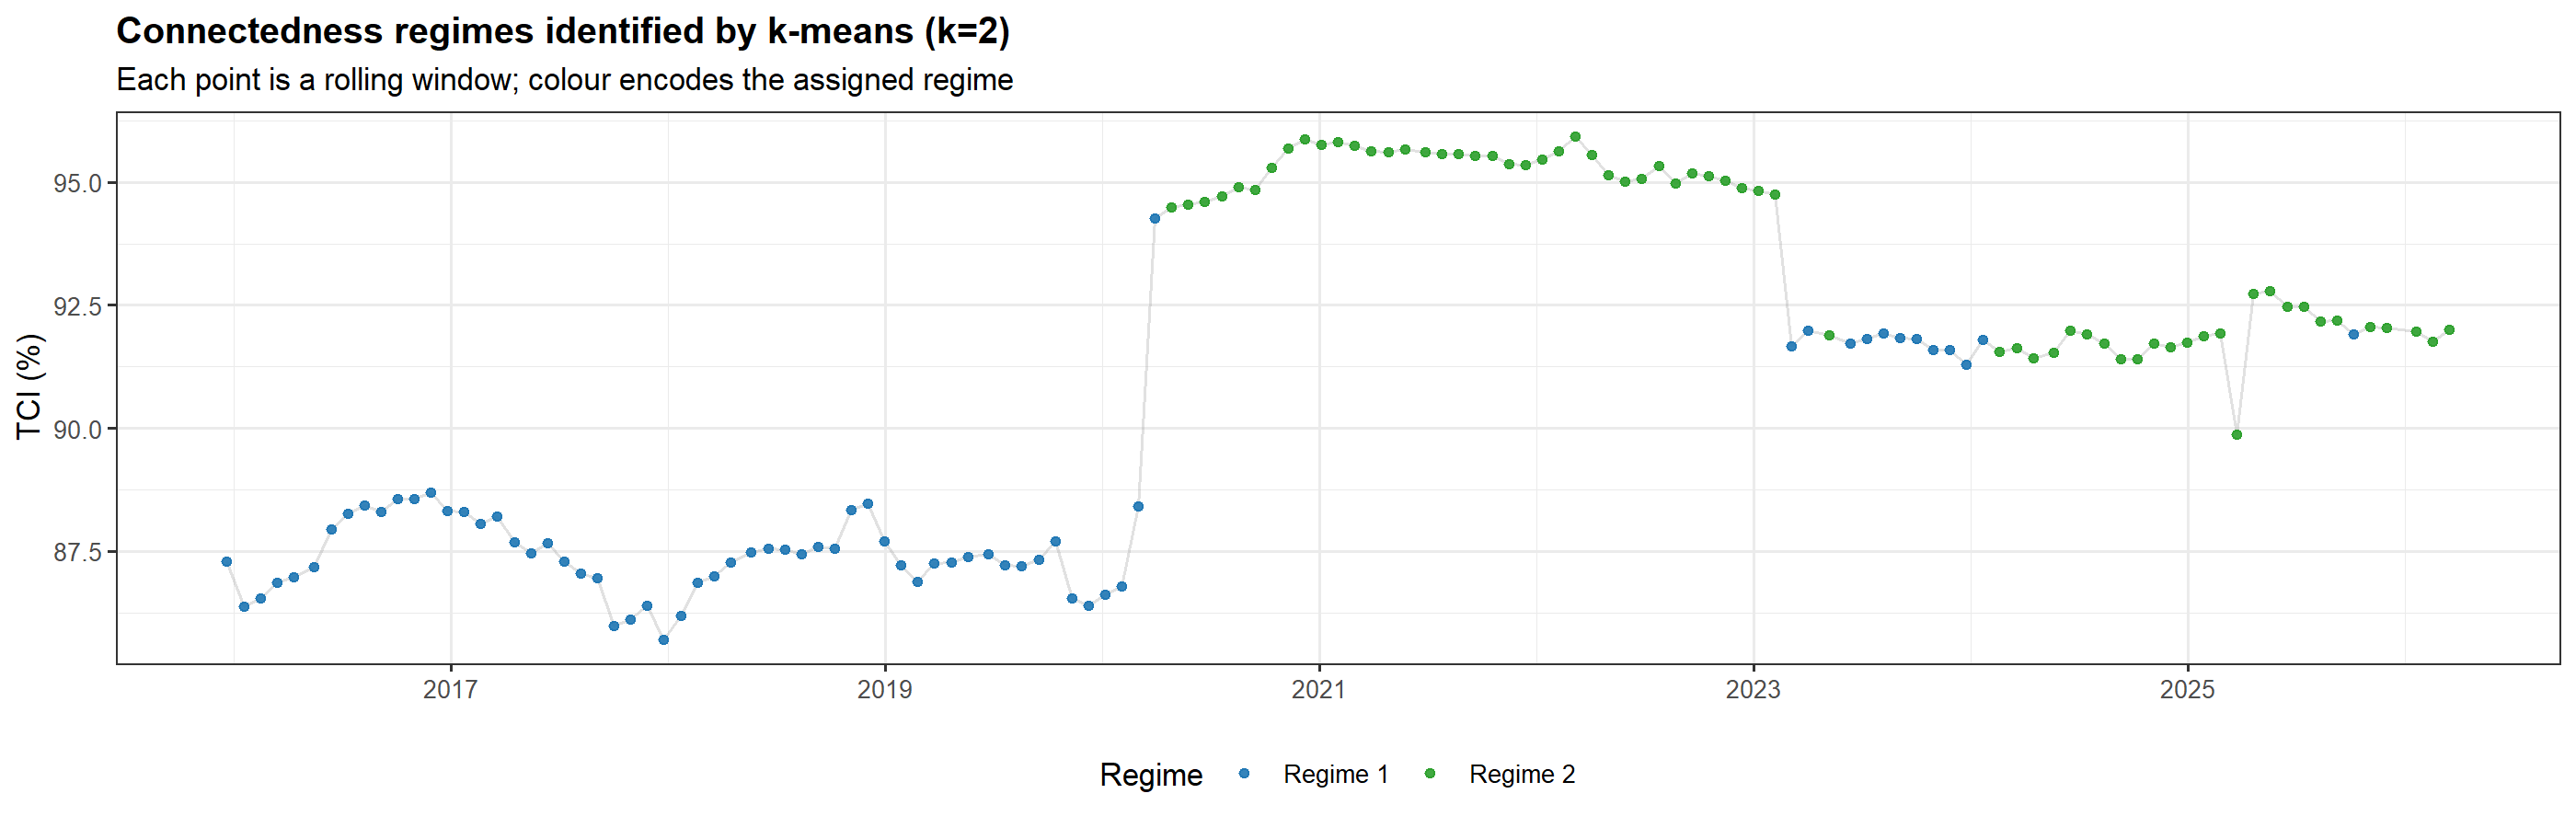
\includegraphics[width=\linewidth,height=0.64\textheight,keepaspectratio]{regime_timeline.png}\\[-1pt]
 % {\color{SlideGray}\tiny $K^{*}=2$ selected by silhouette criterion (mean sil.\,$=0.54$). Features: TCI, $\sigma$(NET), max NET, top-5 TO share, skew(NET).}

%\column{0.41\textwidth}
 % \begin{tcolorbox}[findcard=Accent,width=\linewidth]
    %{\color{Navy}\scriptsize\bfseries Regime 1 — Calm (68 windows)}\\[1pt]
 %   {\color{TextDark}\scriptsize TCI $\approx 88\%$, high dispersion of net spillovers, positive skew. A single dominant transmitter is identifiable.}
  %\end{tcolorbox}
  %\vspace{3pt}
  %\begin{tcolorbox}[findcard=Red,width=\linewidth]
%{\color{Navy}\scriptsize\bfseries Regime 2 — Crisis (64 windows)}\\[1pt]
 %   {\color{TextDark}\scriptsize TCI $\approx 94\%$, \textbf{lower} dispersion, negative skew. Network homogenizes: shocks spread uniformly, dominance of any single transmitter diminishes.}
  %\end{tcolorbox}
  %\vspace{3pt}
  %\begin{tcolorbox}[findcard=Gold,width=\linewidth]
%{\color{Navy}\scriptsize\bfseries Data-Driven Regime Detection}\\[1pt]
 %   {\color{TextDark}\scriptsize Regimes emerge from GFEVD feature vectors without pre-labelling --- the crisis structure is directly identified from the spillover geometry.}
  %\end{tcolorbox}
%\end{columns}
%\end{frame}

% ── SLIDE 12: CROSS-METHOD CENTRALITY ────────────────────────
\begin{frame}{\stag[Green]{Results} Cross-Method Centrality: VAR--DY, MST, and \textcolor {red}{ DCC-GARCH} Networks \textcolor {red}{Full Sample and Time Average??? Why not use Degree for DCC in the right figure??? Clarify the full-sample??? average over windows? }}
\vspace{-1pt}
\begin{columns}[T,onlytextwidth]
\column{0.49\textwidth}
  \centering
  {\color{Navy}\scriptsize\bfseries MST Degree vs.\ VAR--DY Net Spillover}\\[2pt]
  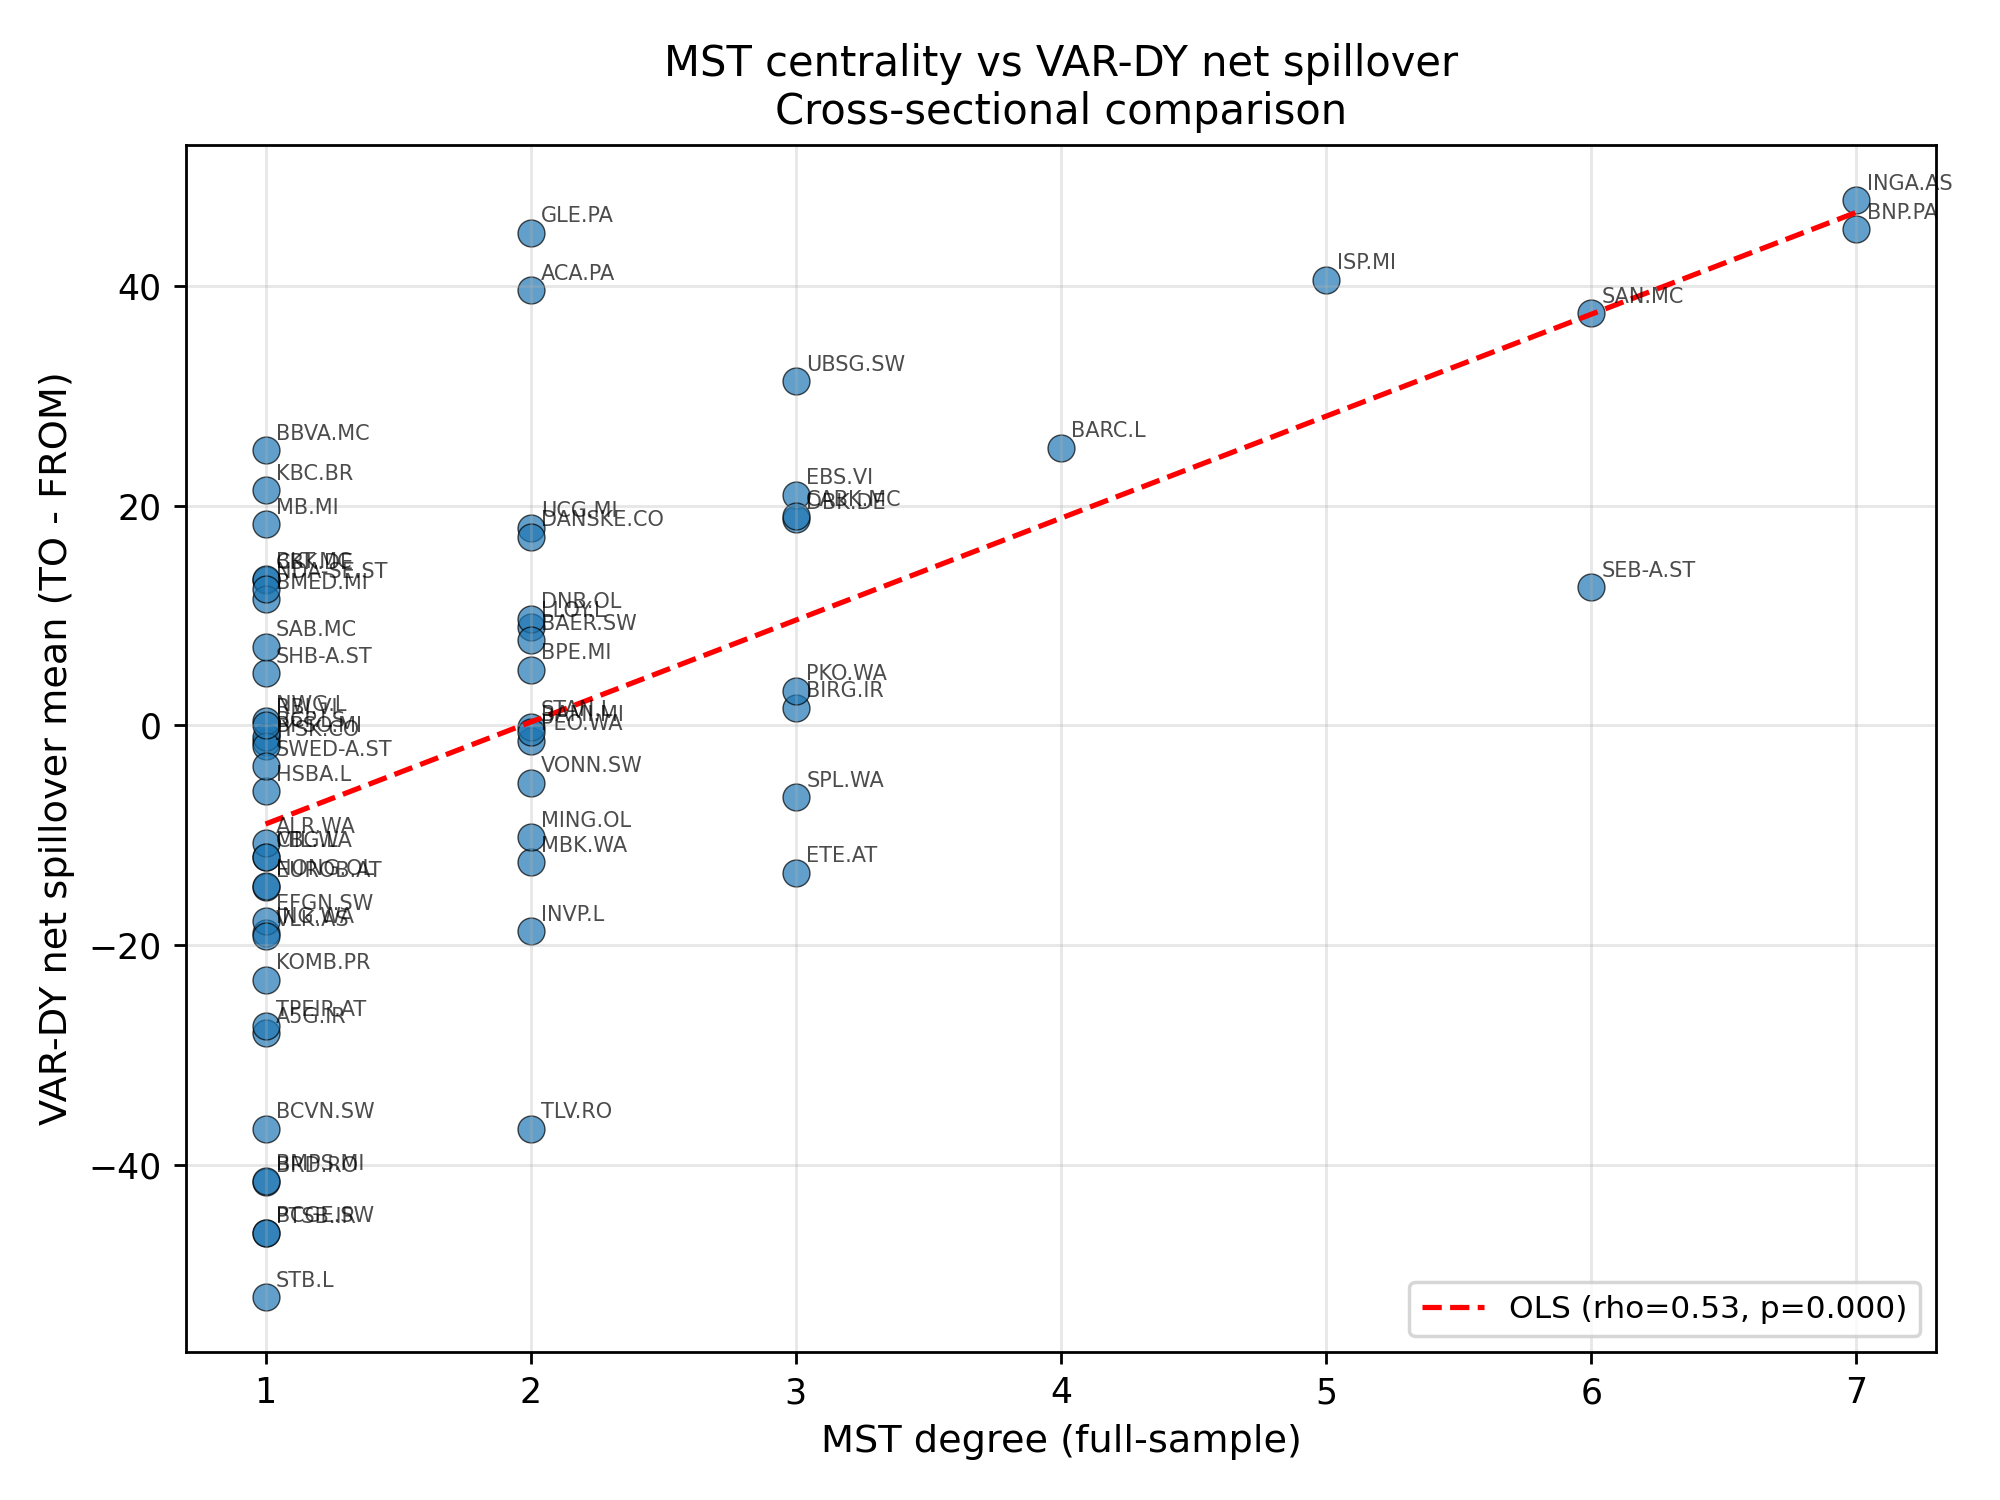
\includegraphics[width=\linewidth,height=0.55\textheight,keepaspectratio]{mst_degree_vs_var_net_scatter.png}\\[-1pt]
  {\color{SlideGray}\tiny Spearman $\rho = 0.53$, $p \approx 0$, $n = 63$}

\column{0.49\textwidth}
  \centering
  {\color{Navy}\scriptsize\bfseries Pearson Eigenvector Centrality vs.\ VAR--DY Net}\\[2pt]
  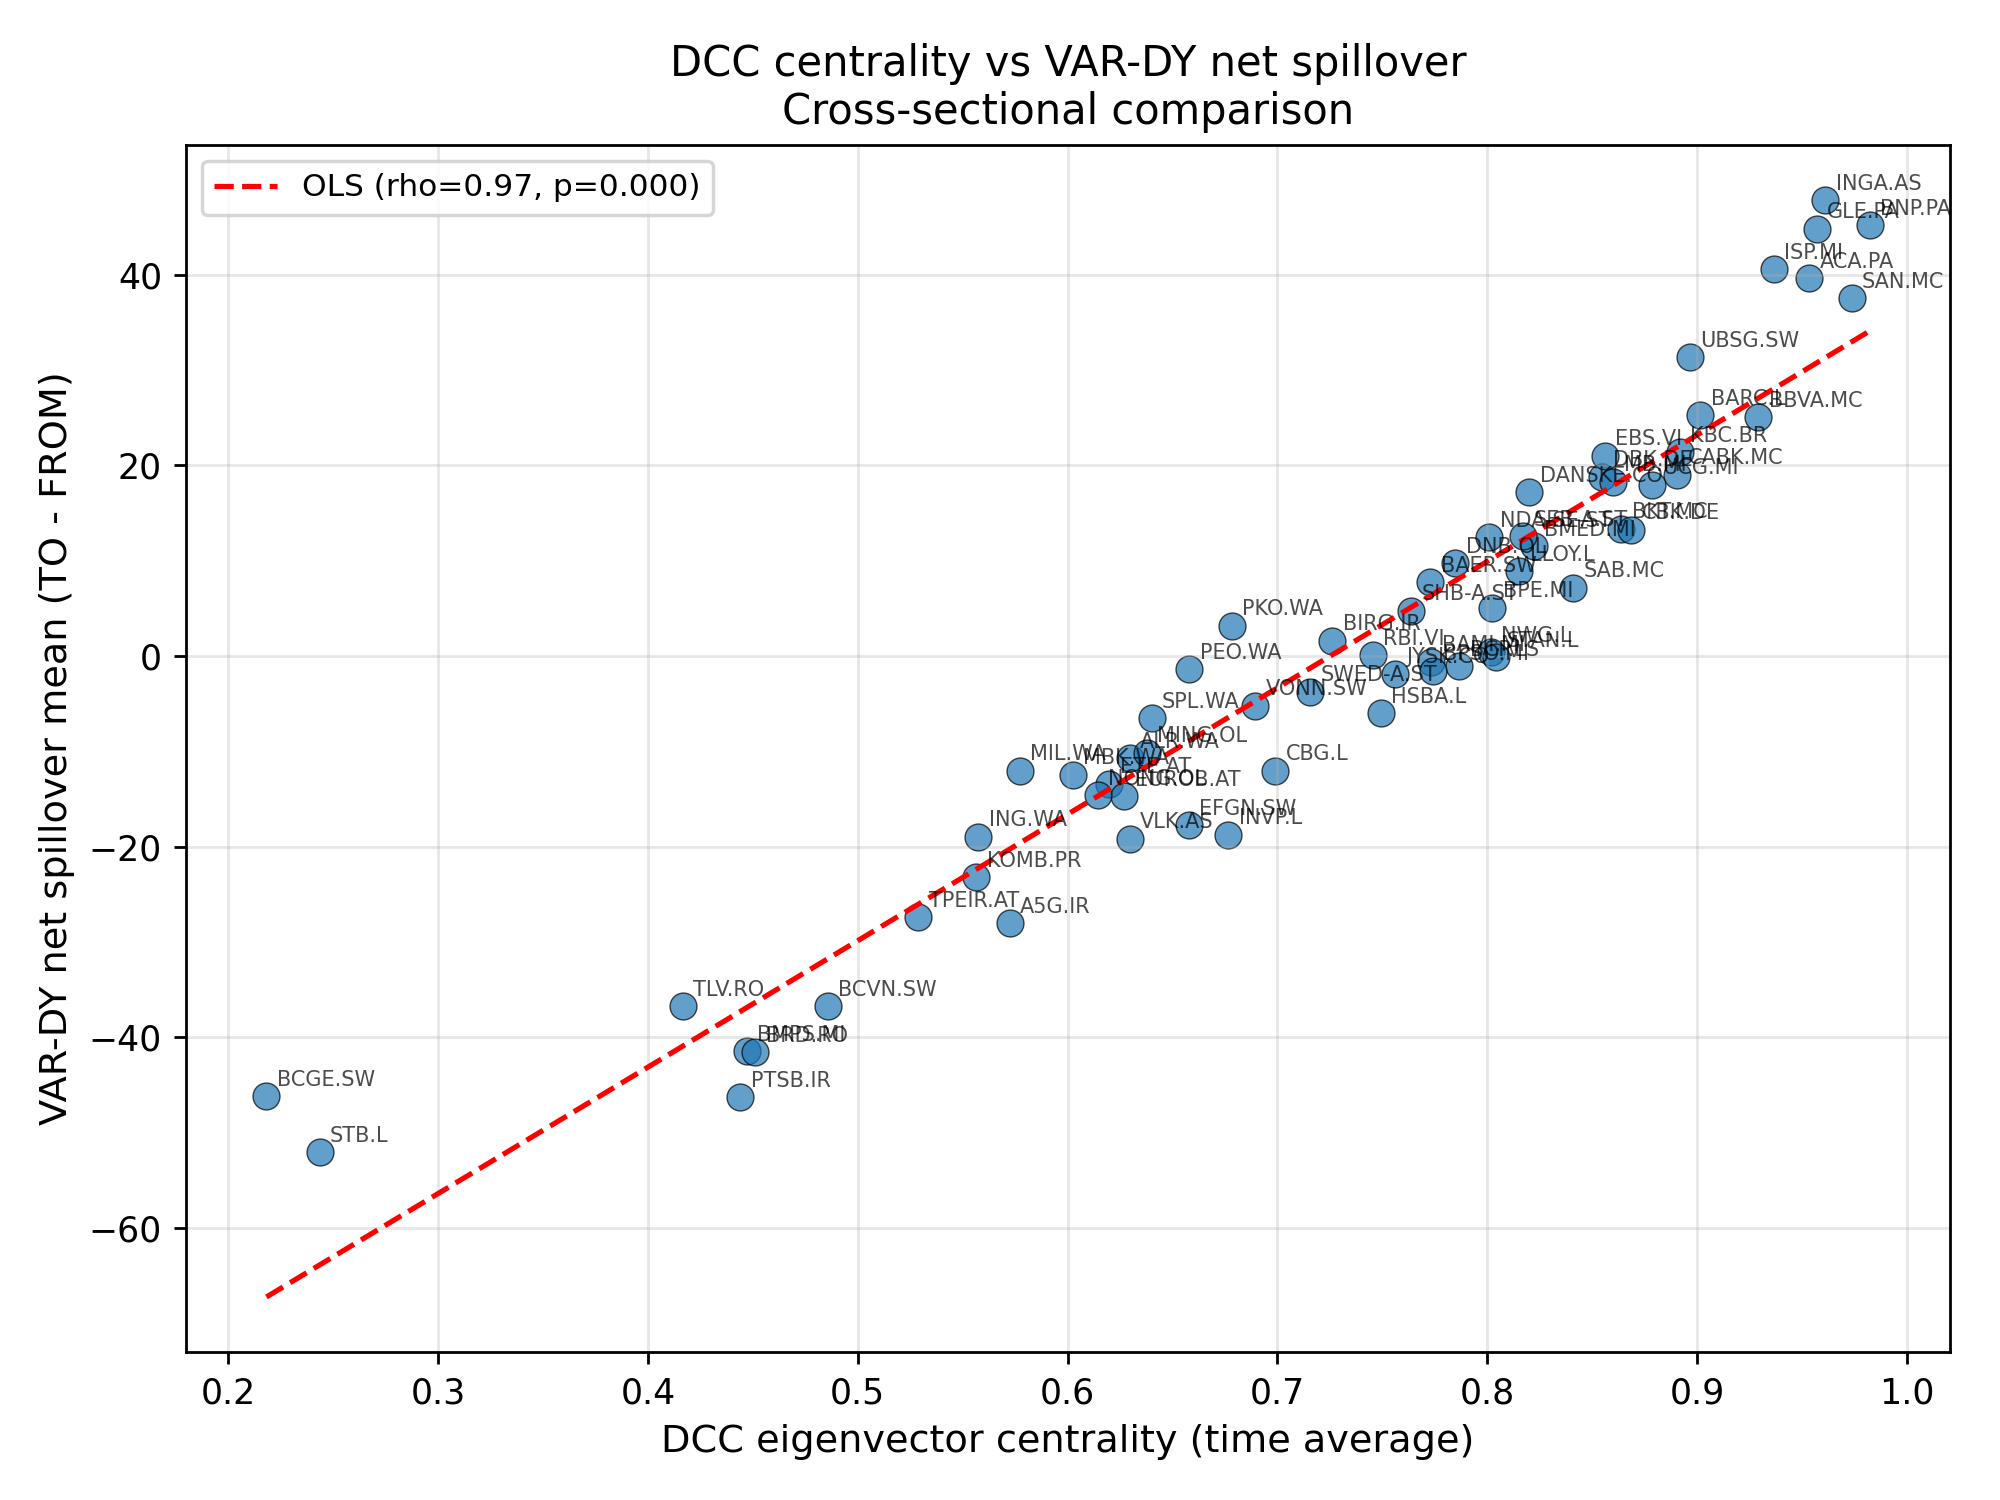
\includegraphics[width=\linewidth,height=0.55\textheight,keepaspectratio]{dcc_eigen_vs_var_net_scatter.png}\\[-1pt]
  {\color{SlideGray}\tiny Spearman $\rho = 0.97$, $p \approx 0$, $n = 63$}
\end{columns}

\vspace{3pt}
\begin{columns}[T,onlytextwidth]
\column{0.32\textwidth}
\begin{tcolorbox}[findcard=Gold,width=\linewidth]
  {\color{Navy}\scriptsize\bfseries MST: moderate alignment}\\[1pt]
  {\color{TextDark}\scriptsize $\rho=0.53$ — spanning-tree topology preserves broad ranking but attenuates intermediate-centrality institutions.}
\end{tcolorbox}

\column{0.32\textwidth}
\begin{tcolorbox}[findcard=Green,width=\linewidth]
  {\color{Navy}\scriptsize\bfseries \textcolor {red}{DCC-GARCH}: near-perfect alignment}\\[1pt]
  {\color{TextDark}\scriptsize $\rho=0.97$ — even raw model-free centrality recovers the same systemic risk hierarchy as VAR--DY.}
\end{tcolorbox}

\column{0.32\textwidth}
\begin{tcolorbox}[findcard=Accent,width=\linewidth]
  {\color{Navy}\scriptsize\bfseries Cross-method robustness}\\[1pt]
  {\color{TextDark}\scriptsize Risk hubs identified by VAR--DY are robust to methodology choice: consistent across econometric and statistical approaches.}
\end{tcolorbox}
\end{columns}
\end{frame}


% ── SLIDEs 12 b,c d: FURTHER COMPARISON ACROSS 3 NETWORKS VAR-DY, DCC-GARCH, MST . PLEASE ADD A SLIDE FOR COMPARISION  ACROSS 3 NETWORKS VAR-DY, DCC-GARCH, MST  HERE


% ── SLIDE 12: CROSS-METHOD CENTRALITY ────────────────────────
\begin{frame}{\stag[Green]{Results} Further  Comparison Across Networks : VAR--DY, MST, and DCC-GARCH} 

PLEASE ADD 3 SLIDES FOR FURTHER  COMPARISION  ACROSS 3 NETWORKS VAR-DY, DCC-GARCH, MST  HERE  (e.g. 3 visualizations of each network with brief summary: overall, they are are the same/similar/different over time? Or detailed pairwise links can be (slightly/strongly/...) different but/and overall metrics (centrality, clustering,...) are similar/different????)
\end{frame}

% ── SLIDE 13: COUNTRY TCI NETWORK ────────────────────────────
\begin{frame}{\stag[Green]{Results} Country-Level TCI Network: Geographical Communities}
\vspace{-1pt}
\begin{tcolorbox}[mathbox,left=4pt,right=4pt,top=2pt,bottom=2pt]
  {\color{Gold}\bfseries\scriptsize Within-country-level TCI:}\quad
  $\displaystyle\mathrm{TCI}_{c,w}=\frac{1}{|G_c|}
   \sum_{i\in G_c}\sum_{\substack{j\in G_c\\j\neq i}}\tilde\theta^g_{ij,w}(H)$
  \quad{\scriptsize where $G_c$ is the set of institutions headquartered in country $c$}
  {\color{Gold}\bfseries\scriptsize Between-country-level TCI:} Similarly, consider bank pairs from two countries
\end{tcolorbox}

\vspace{1pt}
\begin{columns}[T,onlytextwidth]
\column{0.53\textwidth}
  \centering
  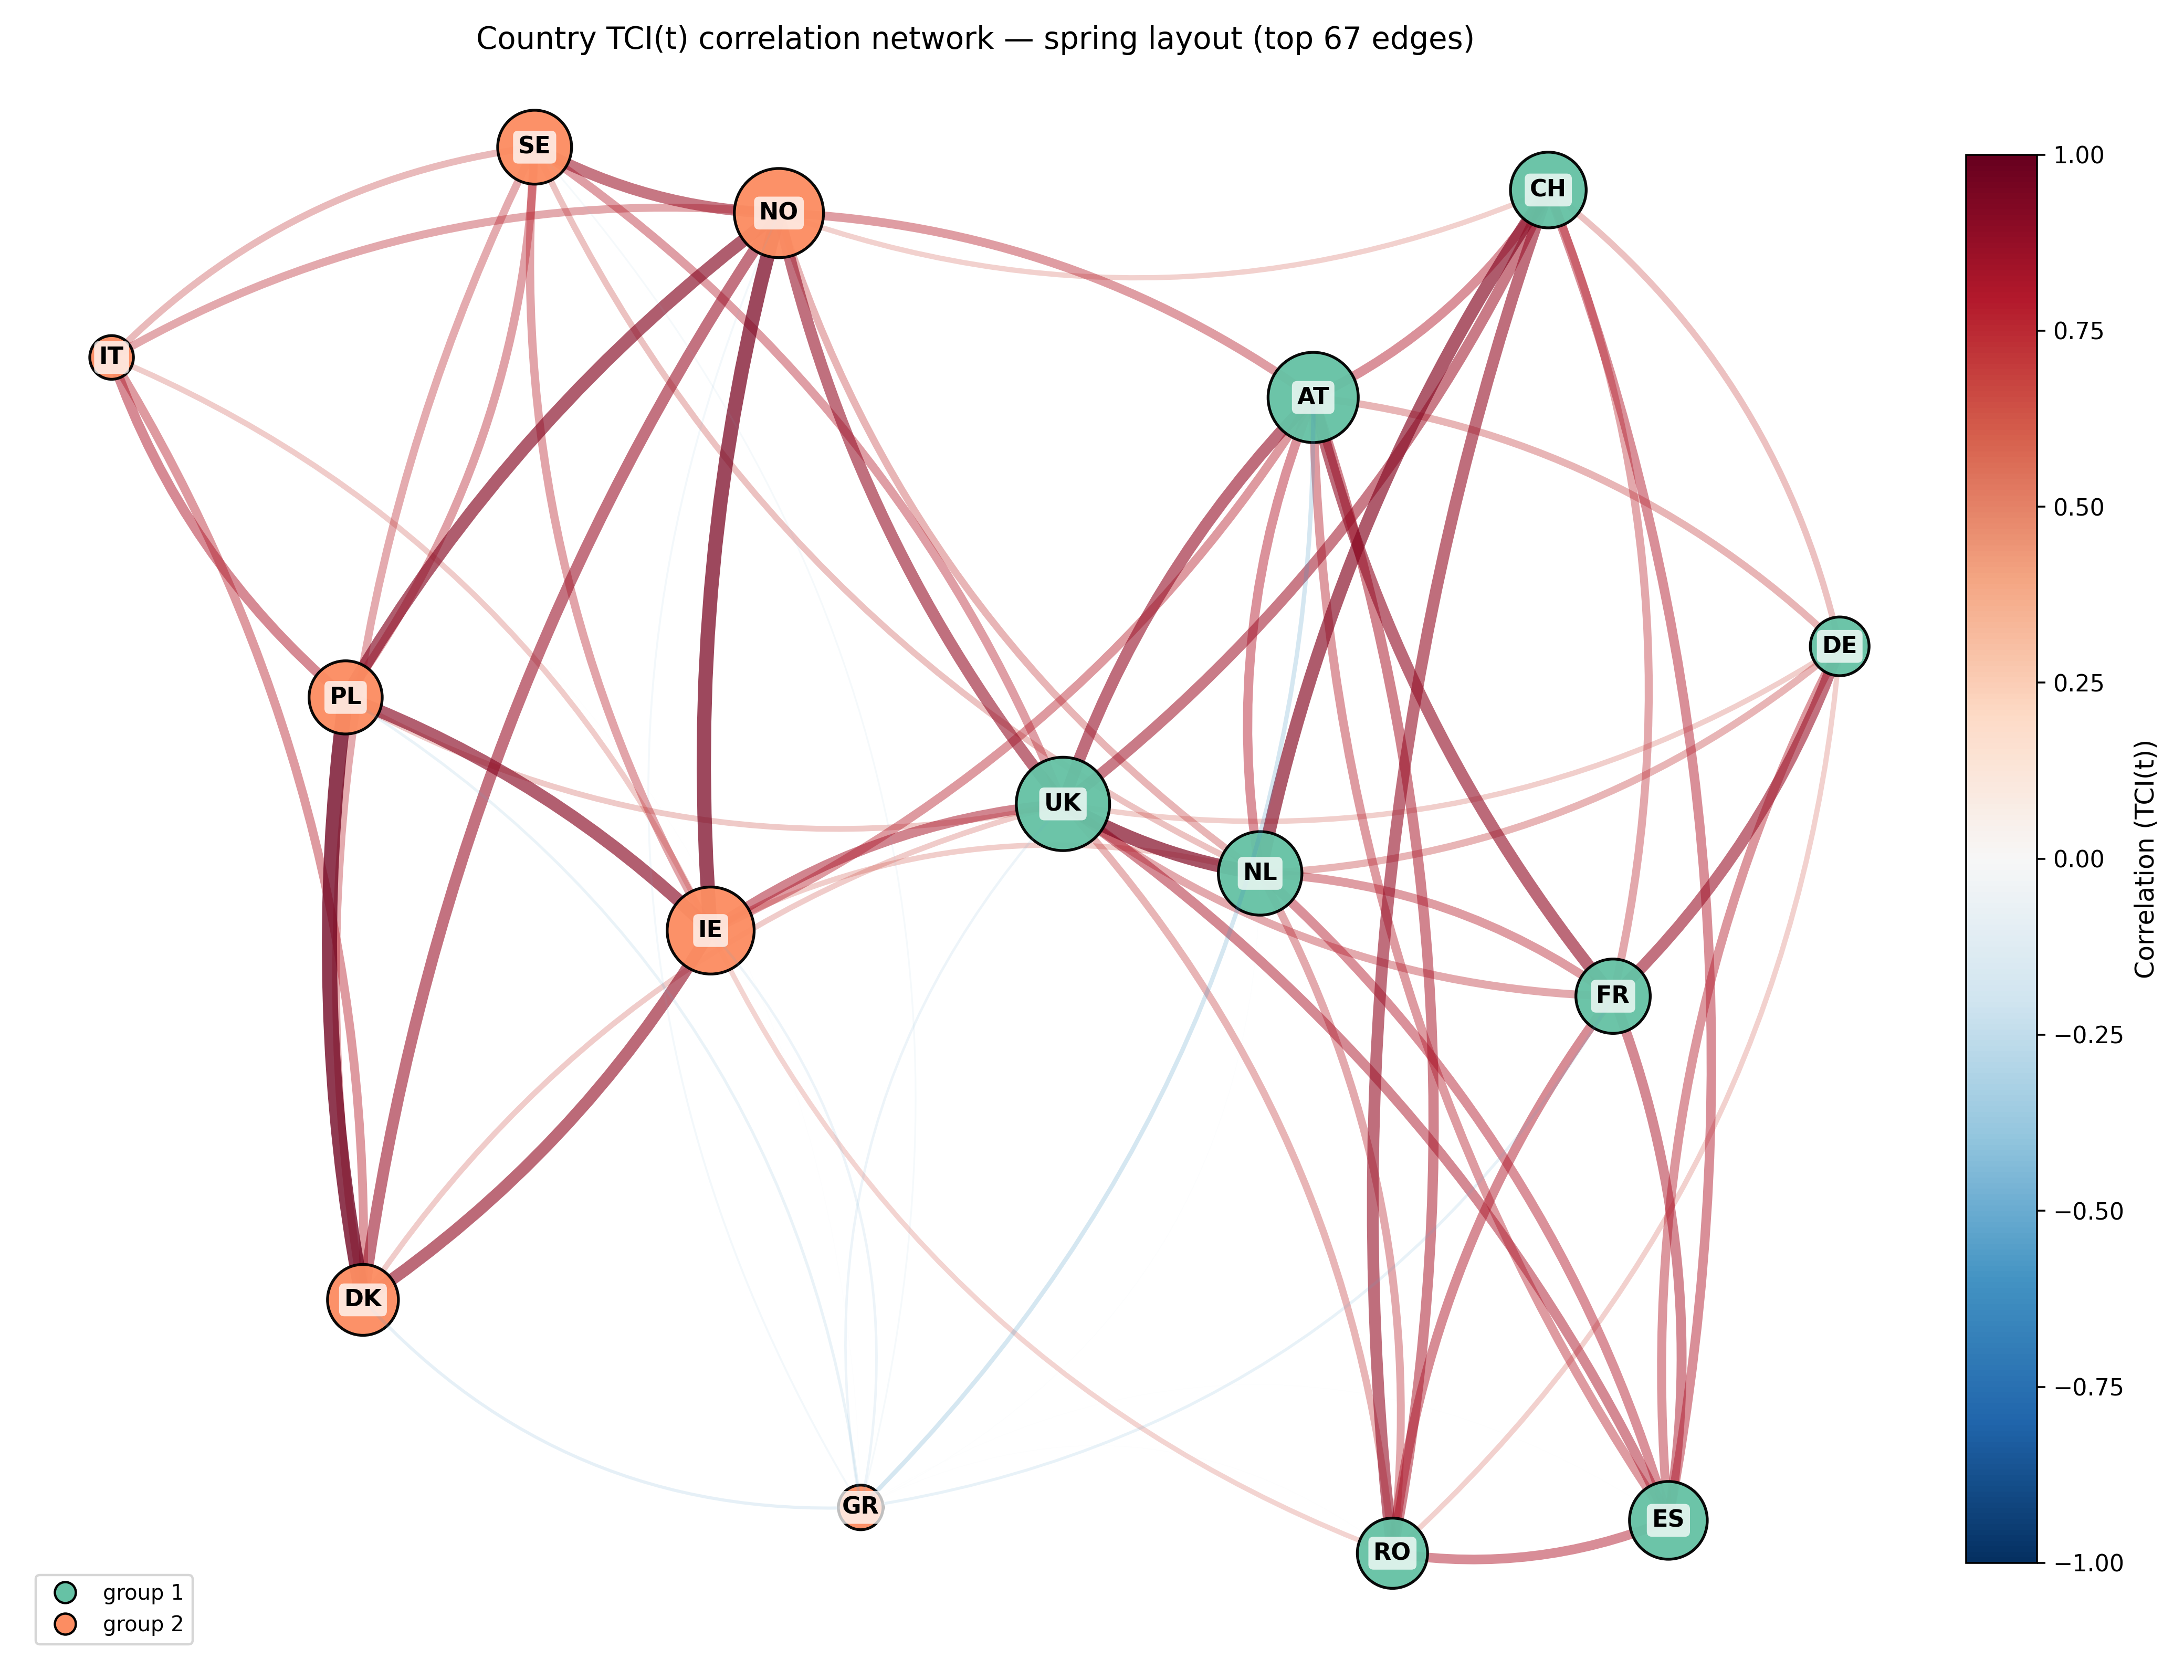
\includegraphics[width=\linewidth,height=0.5\textheight,keepaspectratio]{tci_country_corr_network.png}
  \begin{tcolorbox}[darkstrip,top=0pt,bottom=0pt]
   {\tiny\bfseries Overall Structure:} {\tiny Two large groups but can decompose further into subgroups.}\\
    {\tiny\bfseries Important Implication for Portfolio:} {\tiny cross-community selections, especially in the peripheral and isolated markets (GR/IT/SE), reduces regime lock-in.}
  \end{tcolorbox}
\column{0.45\textwidth}
\vspace{-4pt}
  \begin{tcolorbox}[findcard=Green,width=\linewidth,top=0pt,bottom=0pt]
    {\color{Navy}\scriptsize\bfseries Subgroup 1.1 · Core DE/ES}
    {\color{Green}\scriptsize\bfseries\ DE · ES}\\
    {\color{TextDark}\tiny Core Western Europe; strong mutual spillover co-movement}
  \end{tcolorbox}\vspace{-1pt}
  \begin{tcolorbox}[findcard=Gold,width=\linewidth,top=0pt,bottom=0pt]
    {\color{Navy}\scriptsize\bfseries Subgroup 1.2 · Core Western}
    {\color{Gold}\scriptsize\bfseries\ CH · NL · AT · FR · UK · RO}\\
    {\color{TextDark}\tiny Tightly connected; domestic regimes strongly co-move}
  \end{tcolorbox}\vspace{-1pt}
  \begin{tcolorbox}[findcard=Accent,width=\linewidth,top=0pt,bottom=0pt]
    {\color{Navy}\scriptsize\bfseries Subgroup 2 · Secondary}
    {\color{Accent}\scriptsize\bfseries\ IE · PL · DK · NO}\\
    {\color{TextDark}\tiny Secondary cluster linked to the core}
  \end{tcolorbox}\vspace{-1pt}
  \begin{tcolorbox}[findcard=Purple,width=\linewidth,top=0pt,bottom=0pt]
    {\color{Navy}\scriptsize\bfseries Subgroup 3  · Peripheral}
    {\color{Purple}\scriptsize\bfseries\ SE · IT}\\
    {\color{TextDark}\tiny More idiosyncratic domestic dynamics}
  \end{tcolorbox}\vspace{-1pt}
  \begin{tcolorbox}[findcard=Red,width=\linewidth,top=0pt,bottom=0pt]
    {\color{Navy}\scriptsize\bfseries Subgroup 4 · Isolated}
    {\color{Red}\scriptsize\bfseries\ GR}\\
    {\color{TextDark}\tiny Near-zero or negative TCI correlations; uniquely idiosyncratic}
  \end{tcolorbox}
  %\vspace{-1pt}
  %\begin{tcolorbox}[darkstrip,top=0pt,bottom=0pt]
   % {\tiny\bfseries Portfolio:} {\tiny GR/SE cross-community exposure reduces regime lock-in.}
  %\end{tcolorbox}
\end{columns}
\end{frame}

% ── SLIDE 14: ROBUSTNESS ─────────────────────────────────────
\begin{frame}{\stag[Purple]{Robustness} Robustness: Sensitivity Along Three Dimensions}
\vspace{-1pt}
\begin{columns}[T,onlytextwidth]
\column{0.49\textwidth}
  \begin{tcolorbox}[whitebox=Accent]
    {\color{Navy}\small\bfseries VAR Order $p$}
    \hfill{\color{white}\scriptsize\colorbox{Green}{\bfseries\ \checkmark Robust\ }}\\[2pt]
    {\color{Accent}\scriptsize\itshape Variants: $p=1$ (baseline) vs.\ $p=2$}\\[2pt]
    {\color{TextDark}\scriptsize Virtually identical TCI dynamics and directional rankings. AIC/BIC consistently prefer $p=1$. Companion-matrix stability holds in both cases $\to$ VMA ($\infty$) representation exists.}
  \end{tcolorbox}
  \vspace{3pt}
  \begin{tcolorbox}[whitebox=Accent]
    {\color{Navy}\small\bfseries Forecast Horizon $H$}
    \hfill{\color{white}\scriptsize\colorbox{Green}{\bfseries\ \checkmark Robust\ }}\\[2pt]
    {\color{Accent}\scriptsize\itshape Variants: $H\in\{4,6, 8, 10,12\}$ weeks}\\[2pt]
    {\color{TextDark}\scriptsize TCI levels decrease slightly at shorter horizons, but rankings and time-variation patterns remain similar.}
  \end{tcolorbox}

\column{0.49\textwidth}
  \begin{tcolorbox}[whitebox=Accent]
    {\color{Navy}\small\bfseries Rolling Window $W$}
    \hfill{\color{white}\scriptsize\colorbox{Green}{\bfseries\ \checkmark Robust\ }}\\[2pt]
    {\color{Accent}\scriptsize\itshape Variants: $W\in\{104,156,208\}$ weeks}\\[2pt]
    {\color{TextDark}\scriptsize COVID spike, persistent elevation, and institution ranking are preserved. Shorter windows amplify fluctuations; longer windows smooth them.}
  \end{tcolorbox}
  \vspace{3pt}
  \begin{tcolorbox}[whitebox=Accent]
    {\color{Navy}\small\bfseries DY--DCC Relationship}
    \hfill{\color{white}\scriptsize\colorbox{Green}{\bfseries\ \checkmark Robust\ }}\\[2pt]
    {\color{Accent}\scriptsize\itshape All specifications above}\\[2pt]
    {\color{TextDark}\scriptsize Near-linear association between VAR--DY TCI and DCC mean correlation is preserved throughout: $r>0.90$ in all cases.}
  \end{tcolorbox}
\end{columns}
\end{frame}

% ── SLIDE 15: CONCLUSION ─────────────────────────────────────
{
\setbeamercolor{background canvas}{bg=Navy}
\begin{frame}[plain]
\vspace{0.10cm}
{\color{Accent}\hrule height 0.5pt}
\vspace{0.08cm}
{\color{white}\large\bfseries Conclusion}
\vspace{0.10cm}

\begin{columns}[T,onlytextwidth]
\column{0.49\textwidth}
  \begin{tcolorbox}[enhanced,colback=DarkBlue,colframe=DarkBlue,
    coltext=white,boxrule=0pt,arc=3pt,
    left=5pt,right=5pt,top=3pt,bottom=3pt]
    {\color{Gold}\Large\bfseries 01}\quad{\color{LightBlue}\small\bfseries High Systemic Connectedness}\\[2pt]
    {\scriptsize TCI stays in the upper-80s and surges to about $95\%$ during COVID-19, then remains structurally elevated.}
  \end{tcolorbox}
\column{0.49\textwidth}
  \begin{tcolorbox}[enhanced,colback=DarkBlue,colframe=DarkBlue,
    coltext=white,boxrule=0pt,arc=3pt,
    left=5pt,right=5pt,top=3pt,bottom=3pt]
    {\color{Gold}\Large\bfseries 02}\quad{\color{LightBlue}\small\bfseries Core vs.\ Periphery Asymmetry}\\[2pt]
    {\scriptsize Large cross-border banks dominate as receivers and emitters, while peripheral-market banks remain persistent net transmitters.}
  \end{tcolorbox}
\end{columns}


\vspace{3pt}

\begin{columns}[T,onlytextwidth]
\column{0.49\textwidth}
  \begin{tcolorbox}[enhanced,colback=DarkBlue,colframe=DarkBlue,
    coltext=white,boxrule=0pt,arc=3pt,
    left=5pt,right=5pt,top=3pt,bottom=3pt]
    {\color{Gold}\Large\bfseries 03}\quad{\color{LightBlue}\small\bfseries  Macroprudential Implications}\\[2pt]
    {\scriptsize Not an easy task: Not simply ``Too Big To Fail" or ``Too Small To Matter". Highly interconnected and correlated nature of the network, combined with the heterogeneous roles of individual banks, makes the situation far more complicated!}
  \end{tcolorbox}
\column{0.49\textwidth}
  \begin{tcolorbox}[enhanced,colback=DarkBlue,colframe=DarkBlue,
    coltext=white,boxrule=0pt,arc=3pt,
    left=5pt,right=5pt,top=3pt,bottom=3pt]
    {\color{Gold}\Large\bfseries 04}\quad{\color{LightBlue}\small\bfseries Geographic Diversification}\\[2pt]
    {\scriptsize The country TCI network reveals two main groups with five interconnected sub-communities of countries. Spillovers occur not only within borders but also across them.\\
    However, good news for investors: cross-community portfolios, including GR/IT/SE in the peripheral, may somewhat reduce regime lock-in.}
  \end{tcolorbox}
\end{columns}
\end{frame}
}


% ── SLIDE 15: CONCLUSION ─────────────────────────────────────
{
\setbeamercolor{background canvas}{bg=Navy}
\begin{frame}[plain]
\vspace{0.10cm}
{\color{Accent}\hrule height 0.5pt}
\vspace{0.08cm}
{\color{white}\large\bfseries Future Directions}
\vspace{0.10cm}

\begin{columns}[T,onlytextwidth]
\column{0.49\textwidth}
  \begin{tcolorbox}[enhanced,colback=DarkBlue,colframe=DarkBlue,
    coltext=white,boxrule=0pt,arc=3pt,
    left=5pt,right=5pt,top=3pt,bottom=3pt]
    {\color{Gold}\Large\bfseries 01}\quad{\color{LightBlue}\small\bfseries Future Direction 1}\\[2pt]
    {\scriptsize More detailed comparison accross networks using different local/mesoscale/global network metrics.}
  \end{tcolorbox}
\column{0.49\textwidth}
  \begin{tcolorbox}[enhanced,colback=DarkBlue,colframe=DarkBlue,
    coltext=white,boxrule=0pt,arc=3pt,
    left=5pt,right=5pt,top=3pt,bottom=3pt]
    {\color{Gold}\Large\bfseries 02}\quad{\color{LightBlue}\small\bfseries Future Direction 2}\\[2pt]
    {\scriptsize Consider other types of linkages among European financial institutions, such as interbank relationships, overapping portfolios, derivative exposures, fixed income transactions, foreign exchange (forex) transactions, and other financial exposures.}
  \end{tcolorbox}
\end{columns}

\vspace{3pt}

\begin{columns}[T,onlytextwidth]
\column{0.49\textwidth}
  \begin{tcolorbox}[enhanced,colback=DarkBlue,colframe=DarkBlue,
    coltext=white,boxrule=0pt,arc=3pt,
    left=5pt,right=5pt,top=3pt,bottom=3pt]
    {\color{Gold}\Large\bfseries 03}\quad{\color{LightBlue}\small\bfseries Future Direction 3}\\[2pt]
    {\scriptsize Draw implications for system-wide stress testing.}
  \end{tcolorbox}
\column{0.49\textwidth}
  \begin{tcolorbox}[enhanced,colback=DarkBlue,colframe=DarkBlue,
    coltext=white,boxrule=0pt,arc=3pt,
    left=5pt,right=5pt,top=3pt,bottom=3pt]
    {\color{Gold}\Large\bfseries 04}\quad{\color{LightBlue}\small\bfseries Future Direction 4}\\[2pt]
    {\scriptsize Draw implications for investors, e.g., network-based portfolios.}
  \end{tcolorbox}
\end{columns}
\end{frame}
}
\end{document}